% Thrust 1 progress report: adjusted claims, proposed pipeline, pilot evidence.
% Compile on Overleaf with pdfLaTeX. Figures come from figures4papers/figure_Thrust1UQ/plot_report.py.
\documentclass[aspectratio=169,11pt]{beamer}
\usetheme[progressbar=frametitle,numbering=fraction,block=fill]{metropolis}

\usepackage[utf8]{inputenc}
\usepackage{amsmath,amssymb,bm}
\usepackage{graphicx}
\usepackage{booktabs,array}
\usepackage{xcolor}
\graphicspath{{figures/}}

% Colours shared with the figures (figures4papers palette).
\definecolor{ourblue}{HTML}{0F4D92}
\definecolor{thrustred}{HTML}{B64342}
\definecolor{ink}{HTML}{272727}
\definecolor{inkgrey}{HTML}{767676}
\setbeamercolor{alerted text}{fg=thrustred}
\setbeamercolor{block title}{bg=ourblue!15,fg=black}
\setbeamercolor{block body}{bg=ourblue!4}

\newenvironment{thrustcol}{%
  \setbeamercolor{block title}{bg=thrustred!16,fg=black}%
  \setbeamercolor{block body}{bg=thrustred!4}%
  \begin{block}{Thrust 1 as written}}{\end{block}}
\newenvironment{ourcol}{%
  \setbeamercolor{block title}{bg=ourblue!16,fg=black}%
  \setbeamercolor{block body}{bg=ourblue!4}%
  \begin{block}{Our proposal}}{\end{block}}

\newcommand{\E}{\mathbb{E}}
\newcommand{\Var}{\mathrm{Var}}
\newcommand{\x}{\bm{x}}
\newcommand{\D}{\bm{D}}
\newcommand{\Ft}{\bm{F}_\theta}
\newcommand{\source}[1]{\par\vfill{\scriptsize\color{inkgrey}#1}}

\title{Uncertainty in Compiled Feature Flows}
\subtitle{Adjusted claims of Thrust 1, a proposed pipeline, and pilot evidence}
\author{Your Name}
\institute{Progress report, meeting with Prof.~Nghia}
\date{\today}

\begin{document}

\maketitle

% ============================================================
\begin{frame}{We keep the Thrust 1 backbone and change its uncertainty layer}
  \begin{enumerate}
    \item \textbf{Adjusted claims.} Eight statements of Section 3.2, each placed next to the version we propose, with the derivation that supports it, plus one refinement found at scale.
    \item \textbf{Proposed pipeline.} Compile the FM as in Task 1, then attach a regeneration scaffold that keeps every layer marginal exactly, has a closed-form predictive, and carries a conformal flip guarantee.
    \item \textbf{Evidence at three scales.} Six pilot experiments on a 4-block ViT (digits, 5 splits), then the full ablation ladder with ViT-B/16 on CIFAR-10 and CIFAR-100 (DIRECTOR setting) and on ImageNet.
  \end{enumerate}
  \smallskip
  {\small Notation: $p_l$ is the feature distribution after layer $l$ under the data distribution $p_0$; $L$ is the number of layers that carry uncertainty; $p(y\mid\x)$ is the FM prediction.}
\end{frame}

% ============================================================
\begin{frame}{Thrust 1 and our proposal share the same backbone}
  \begin{columns}[T,onlytextwidth]
    \column{0.485\textwidth}
    \begin{thrustcol}
      \small
      \begin{enumerate}
        \item Compile blocks into $\Ft(\x,t)$ by flow matching (Eq.~3, 7).
        \item Brownian scaffold $g$ with score drift (Eq.~5).
        \item Variance prior from a score-weighted penalty (Eq.~8).
        \item Per-input uncertainty by a quadrature recursion (Eq.~6).
        \item Scaffold refinement by a Wasserstein bound (Eq.~9).
      \end{enumerate}
    \end{thrustcol}
    \column{0.485\textwidth}
    \begin{ourcol}
      \small
      \begin{enumerate}
        \item Same compilation, plus a Gronwall fidelity certificate.
        \item Regeneration kernel: exact marginal, no score model.
        \item Jump rate from layer distances with a conformal threshold.
        \item Closed-form predictive from the first-jump decomposition.
        \item Finite-class Hoeffding (or PAC-Bayes) bound on held-out data.
      \end{enumerate}
    \end{ourcol}
  \end{columns}
  \smallskip
  {\small Items 2 to 5 replace components whose stated guarantees do not hold as written (next section). Item 1 is unchanged.}
\end{frame}

% ============================================================
\begin{frame}{Our pipeline keeps the compiled flow and replaces the scaffold}
  \centering
  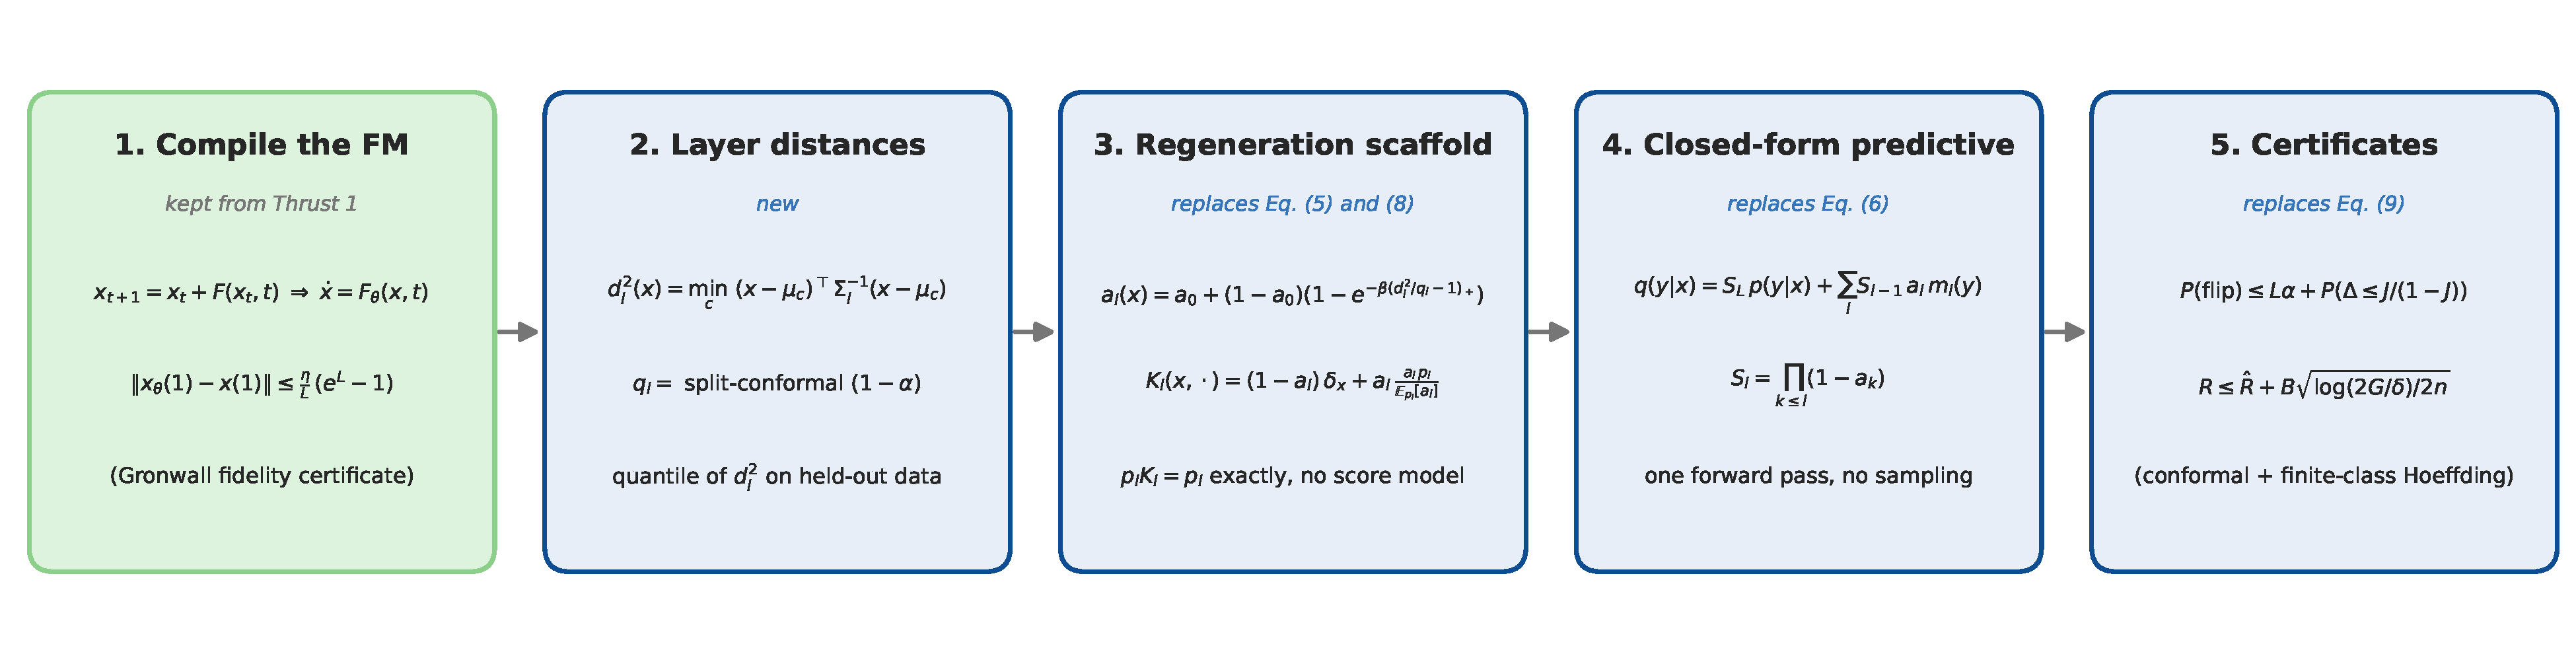
\includegraphics[width=\linewidth]{fig_pipeline.pdf}
  \par\medskip
  \raggedright\small
  Green: kept from Thrust 1. Blue: new components. Every box states the identity or bound it relies on; the derivations follow on the next slides.
\end{frame}

% ============================================================
\section{Adjusted claims}

\begin{frame}{Compilation is kept and gains a fidelity certificate}
  \begin{columns}[T,onlytextwidth]
    \column{0.44\textwidth}
    \begin{thrustcol}
      \small
      Residual blocks $\x_{t+1}=\x_t+F(\x_t,t)$ are distilled into one field $\Ft(\x,t)$ by amortized flow matching (Eq.~7). Fidelity of the compiled ODE to the FM is not quantified.
    \end{thrustcol}
    \column{0.53\textwidth}
    \begin{ourcol}
      \small
      Keep Eq.~(7). If $\|\Ft(\x,t)-F(\x,t)\|\le\eta$ and $F$ is $L_F$-Lipschitz in $\x$, the error $e(t)=\|\x_\theta(t)-\x(t)\|$ obeys
      \[
        \dot e\le \eta+L_F\,e,\quad e(0)=0
        \;\Rightarrow\;
        e(1)\le \frac{\eta}{L_F}\big(e^{L_F}-1\big)
      \]
      (Gronwall). With an $L_h$-Lipschitz head, the logit gap is at most $L_h\,e(1)$.
      \smallskip

      \textbf{Use:} report argmax agreement and $e(1)$ of the compiled ODE before any uncertainty is added (rung 2 of the ablation ladder).
    \end{ourcol}
  \end{columns}
\end{frame}

% ============================================================
\begin{frame}{Preserving the marginal does not preserve each input}
  \begin{columns}[T,onlytextwidth]
    \column{0.44\textwidth}
    \begin{thrustcol}
      \small
      The SDE of Eq.~(5) ``preserves the feature distribution and hence the representation entropy'', so $g$ can be designed ``without affecting the FM's representation structure''.
    \end{thrustcol}
    \column{0.53\textwidth}
    \begin{ourcol}
      \small
      With $p_1$ fixed, two identities hold for any scaffold:
      \[
        \underbrace{\Var[\x(1)]}_{\text{fixed}}=\E\,\Var[\x(1)\mid\x_0]+\Var\,\E[\x(1)\mid\x_0],
      \]
      \[
        \underbrace{H(\x(1))}_{\text{fixed}}=H(\x(1)\mid\x_0)+I(\x_0;\x(1)).
      \]
      Uncertainty added by the scaffold is paid for by shrinking the conditional means and losing mutual information with the input.
      \smallskip

      \textbf{Consequence:} spend the budget only where $p_0$ has little mass, where the constraint costs almost nothing.
    \end{ourcol}
  \end{columns}
\end{frame}

% ============================================================
\begin{frame}{A state-dependent scaffold needs a divergence term}
  \begin{columns}[T,onlytextwidth]
    \column{0.44\textwidth}
    \begin{thrustcol}
      \small
      \[
        \bm G=\Ft+\tfrac12\,\bm g\bm g^\top\nabla\log p_t,
      \]
      with $\frac{d}{dt}\log p_t(\x(t))=-\operatorname{div}\Ft$ stated along the SDE.
    \end{thrustcol}
    \column{0.53\textwidth}
    \begin{ourcol}
      \small
      With $\D=\bm g\bm g^\top$, the Fokker-Planck equation gives
      \[
        \partial_t p=-\nabla\!\cdot\!\big[(\bm G-\tfrac12\D\nabla\log p-\tfrac12\nabla\!\cdot\!\D)\,p\big],
      \]
      so $p_t$ matches the ODE marginal when
      \[
        \bm G=\Ft+\tfrac12\D\nabla\log p_t+\tfrac12\nabla\!\cdot\!\D .
      \]
      The log-density identity holds along ODE characteristics, not along SDE paths (It\^o terms appear).
      \smallskip

      \textbf{Check:} without the term the marginal variance drops from $1$ to $0.53$.
    \end{ourcol}
  \end{columns}
\end{frame}

% ============================================================
\begin{frame}{Regeneration preserves the marginal without a score model}
  \begin{columns}[T,onlytextwidth]
    \column{0.40\textwidth}
    \begin{thrustcol}
      \small
      Brownian scaffold $g$ with drift correction $\tfrac12\D\nabla\log p_t$: a score model of every $p_t$ is required, and it is least accurate off the data, where it matters most.
    \end{thrustcol}
    \column{0.57\textwidth}
    \begin{ourcol}
      \small
      For a jump probability $a(\x)\in[0,1]$, define
      \[
        K(\x,A)=\big(1-a(\x)\big)\mathbf 1_A(\x)+a(\x)\,\frac{\int_A a\,p}{\E_p[a]} .
      \]
      Then for every measurable $A$,
      \[
        \int p(\x)K(\x,A)\,d\x=p(A)-\int_A a\,p+\E_p[a]\,\frac{\int_A a\,p}{\E_p[a]}=p(A).
      \]
      The marginal is preserved exactly for \emph{any} $a$, using samples of $p_l$ only (training features at layer $l$). After a jump the state no longer depends on $\x$ (Markov property).
    \end{ourcol}
  \end{columns}
\end{frame}

% ============================================================
\begin{frame}{Distances with conformal thresholds encode (a), (b) and (c)}
  \begin{columns}[T,onlytextwidth]
    \column{0.37\textwidth}
    \begin{thrustcol}
      \small
      Eq.~(8) weights $\operatorname{tr}(\bm g\bm g^\top)^{-1}$ by $\|\nabla\log p_t\|$. The optimum is $T^\star\approx\sqrt{\lambda\|\nabla\log p_t\|/c}$, which is smallest where the loss curvature $c$ is largest, i.e. on ambiguous inputs.
    \end{thrustcol}
    \column{0.60\textwidth}
    \begin{ourcol}
      \small
      $a_l(\x)=a_0+(1-a_0)\big(1-e^{-\beta(d_l^2(\x)/q_l-1)_+}\big)$, with $d_l$ the class Mahalanobis distance and $q_l$ the split-conformal $(1-\alpha)$ quantile on held-out data.
      \begin{itemize}
        \item[(a)] $d_l^2\le q_l$ for all $l$ $\Rightarrow$ jump mass $J=J_0=1-(1-a_0)^L$.
        \item[(b)] $d_l\to\infty$ $\Rightarrow$ $a_l\to1$ and $q(y\mid\x)$ reverts to a population predictive.
        \item[(c)] Exchangeability: $P(d^2_{\mathrm{new}}>q_l)\le\alpha$. Writing $q=(1-J)\,p+J\,\bar m$ gives $q_{c^\ast}-q_c\ge(1-J)\Delta-J$, so
          \[
            P(\text{flip})\le L\alpha+P\big(\Delta\le J_0/(1-J_0)\big),
          \]
          with $\Delta$ the FM top-2 margin.
      \end{itemize}
    \end{ourcol}
  \end{columns}
\end{frame}

% ============================================================
\begin{frame}{A closed-form predictive replaces the recursion of Eq.~(6)}
  \begin{columns}[T,onlytextwidth]
    \column{0.40\textwidth}
    \begin{thrustcol}
      \small
      Chapman-Kolmogorov recursion with Gauss-Hermite nodes, claimed cost $O(\log(1/\delta)^{1/\epsilon})$ with error $O(\delta)$. In $d$ dimensions a tensor rule needs $N^{d}$ nodes per step, and errors add over $1/\epsilon$ steps.
    \end{thrustcol}
    \column{0.57\textwidth}
    \begin{ourcol}
      \small
      Condition on the first jump. With $S_l=\prod_{k\le l}(1-a_k)$,
      \[
        q(y\mid\x)=S_L\,p(y\mid\x)+\sum_{l=1}^{L}S_{l-1}\,a_l\,m_l(y),
      \]
      where $m_l(y)=\E_{\x'\sim a_lp_l/\E[a_l]}\,q_{>l}(y\mid\x')$ does not depend on $\x$ and is computed once, offline, by a backward recursion over training features.
      \smallskip

      \textbf{Cost:} one forward pass and $L$ distances; no sampling. In continuous time, $q=S(1)\,p+\int_0^1\lambda(\x(\tau))S(\tau)\,m_\tau\,d\tau$, a 1-D integral whose $n$-node trapezoid error is $O(1/n)$ for a Lipschitz integrand, in any dimension.
    \end{ourcol}
  \end{columns}
\end{frame}

% ============================================================
\begin{frame}{Scaffold selection needs a candidate-dependent empirical term}
  \begin{columns}[T,onlytextwidth]
    \column{0.42\textwidth}
    \begin{thrustcol}
      \small
      \[
        \E\,\ell_\phi\le\tfrac1n{\textstyle\sum_i}\ell_\gamma(\x_i,z_i)+\tau_\varphi\,\E\,W_\varphi(p_\phi,p_\gamma)+\varepsilon .
      \]
      Only the Wasserstein term depends on $\phi$, so minimizing the bound returns $\phi=\gamma$: nothing is refined against (c).
    \end{thrustcol}
    \column{0.55\textwidth}
    \begin{ourcol}
      \small
      Finite candidate set $\Phi$ ($|\Phi|=G$), loss $\ell\in[0,B]$, selection split of size $n$ independent of the thresholds. Hoeffding and a union bound give, with probability $\ge1-\delta$, for all $\phi\in\Phi$:
      \[
        R(\phi)\le\hat R_n(\phi)+B\sqrt{\frac{\log(2G/\delta)}{2n}} .
      \]
      For continuous scaffolds, the PAC-Bayes form keeps $\gamma$ as a prior fitted on separate data:
      \[
        R(Q)\le\hat R_n(Q)+\sqrt{\frac{\mathrm{KL}(Q\|P_\gamma)+\log(2\sqrt n/\delta)}{2n}}\quad(\ell\in[0,1]).
      \]
    \end{ourcol}
  \end{columns}
\end{frame}

% ============================================================
\begin{frame}{The target is a population predictive, not the posterior}
  \begin{columns}[T,onlytextwidth]
    \column{0.42\textwidth}
    \begin{thrustcol}
      \small
      The stochastic path is an ``(equivalent)'' re-parameterization of the pushforward of $p(\theta\mid\mathcal D)$ in Eq.~(1).
    \end{thrustcol}
    \column{0.55\textwidth}
    \begin{ourcol}
      \small
      Under a posterior, outputs at two inputs are dependent through the shared $\theta$:
      \[
        \mathrm{Cov}\big(f_\theta(\x_a),f_\theta(\x_b)\big)\neq0 \text{ in general.}
      \]
      A Markov flow run independently for each input gives a joint law that factorizes over inputs, so it cannot equal the pushforward. We therefore claim only:
      \begin{enumerate}
        \item every layer marginal $p_l$ is unchanged;
        \item far from the data the predictive reverts to a population predictive;
        \item in-distribution flips are bounded as on the previous slide.
      \end{enumerate}
    \end{ourcol}
  \end{columns}
\end{frame}

% ============================================================
\begin{frame}{Partitioned regeneration keeps the marginal for any soft partition}
  \begin{columns}[T,onlytextwidth]
    \column{0.42\textwidth}
    \begin{thrustcol}
      \small
      \textbf{Population regeneration} (our first version). With $q=(1-J)\,p+J\,m$,
      \[
        q_y-p_y=J\,(m_y-p_y),
      \]
      so the true class gains mass only if $m_y>p_y$. The population predictive has $m_y\approx1/C$: harmless with $C=9$, costly with $C=1000$.
    \end{thrustcol}
    \column{0.55\textwidth}
    \begin{ourcol}
      \small
      Take any $w_c(\x)\ge0$ with $\sum_c w_c=1$, and regenerate with probability $a(\x)w_c(\x)$ from $a\,w_c\,p/\E_p[a w_c]$. Then
      \[
        \text{inflow}(\x')=\sum_c \E_p[a w_c]\,\frac{a(\x')w_c(\x')p(\x')}{\E_p[a w_c]}=a(\x')p(\x'),
      \]
      which equals the outflow, so $p_l$ is unchanged. We use $w(\x)=\mathrm{softmax}\big(\log p(\cdot\mid\x)/\tau\big)$: $\tau=1$ reverts toward the predicted class, $\tau=\infty$ recovers the population version. The predictive stays closed form:
      \[
        q=S_L\,p+\textstyle\sum_l S_{l-1}\,a_l\,(w_l M_l),
      \]
      with $M_l$ a $C\times C$ matrix computed offline.
    \end{ourcol}
  \end{columns}
\end{frame}

% ============================================================
\section{Pilot evidence}

\begin{frame}{The pilot isolates the uncertainty layer from compilation error}
  \small
  \begin{itemize}
    \item \textbf{Data.} sklearn digits ($8\times8$). Classes 0 to 8 are in distribution. OOD: held-out digit 9, $90^\circ$ rotations, uniform noise. Shift: test digits plus pixel noise ($\sigma=0.3$), labels kept.
    \item \textbf{FM.} 4-block pre-LN ViT, $d=64$, dropout $0.1$, about $98\%$ accuracy. The FM blocks are used directly, so compilation error is zero and only the uncertainty layer is tested.
    \item \textbf{Splits.} 5 random splits (train, validation, test $=60/20/20$). All numbers are mean $\pm$ std over splits.
    \item \textbf{Baselines.} Temperature scaling (TS), MC dropout (32 passes), a deep ensemble (5 models), and the Brownian same-marginal family of Eq.~(5) simulated exactly with MALA.
    \item \textbf{Proposed scaffold.} Layers: blocks 1 to 4 and the final representation $z$ ($L=5$). Thresholds $q_l$ from one half of the validation set; $(\alpha,\beta,a_0)$ chosen by NLL on the other half.
  \end{itemize}
\end{frame}

% ============================================================
\begin{frame}{The variance budget is fixed once the marginal is fixed}
  \centering
  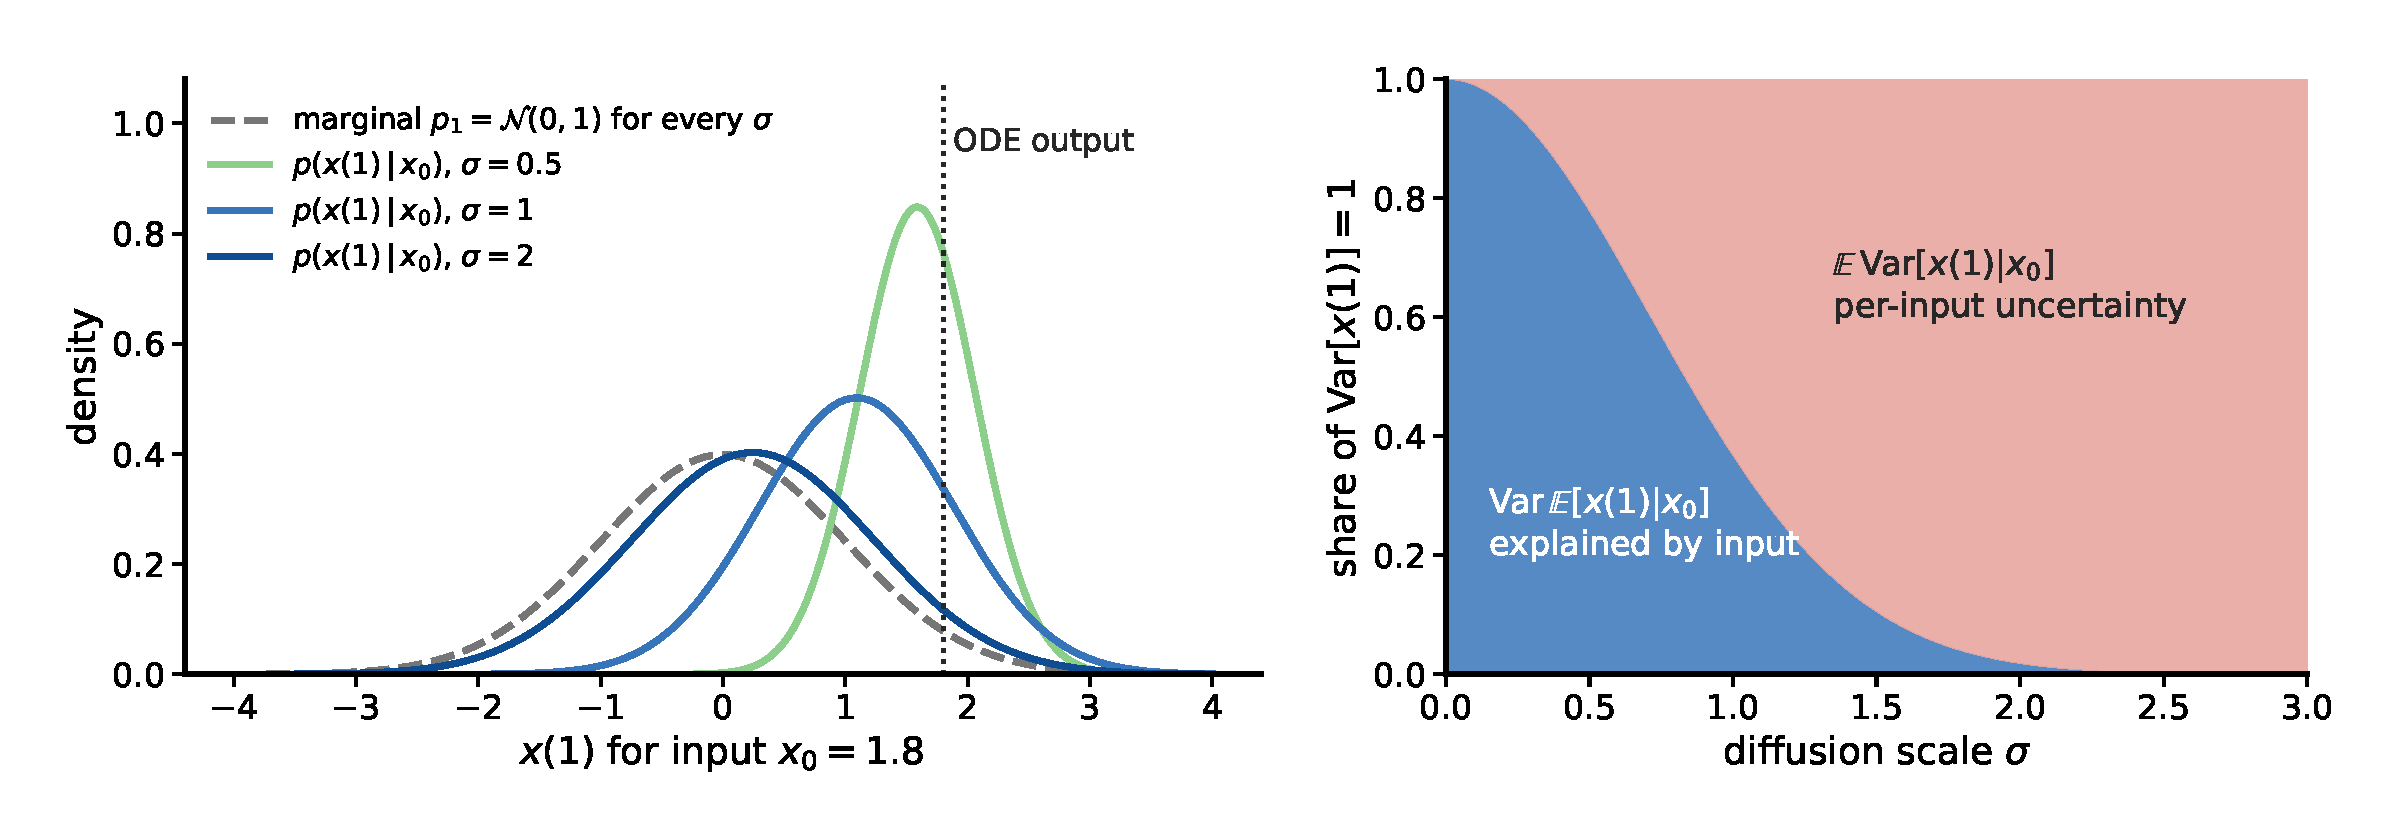
\includegraphics[width=0.92\linewidth]{fig_budget.pdf}
  \par\smallskip\raggedright\small
  Ornstein-Uhlenbeck case of Eq.~(5) with $\Ft=0$, $p_0=\mathcal N(0,1)$, $g=\sigma$: $\E[x(1)\mid x_0]=e^{-\sigma^2/2}x_0$ and $\Var[x(1)\mid x_0]=1-e^{-\sigma^2}$, while $p_1=\mathcal N(0,1)$ for every $\sigma$.
\end{frame}

% ============================================================
\begin{frame}{MC dropout keeps the ID marginal at $z$ and widens it on OOD}
  \centering
  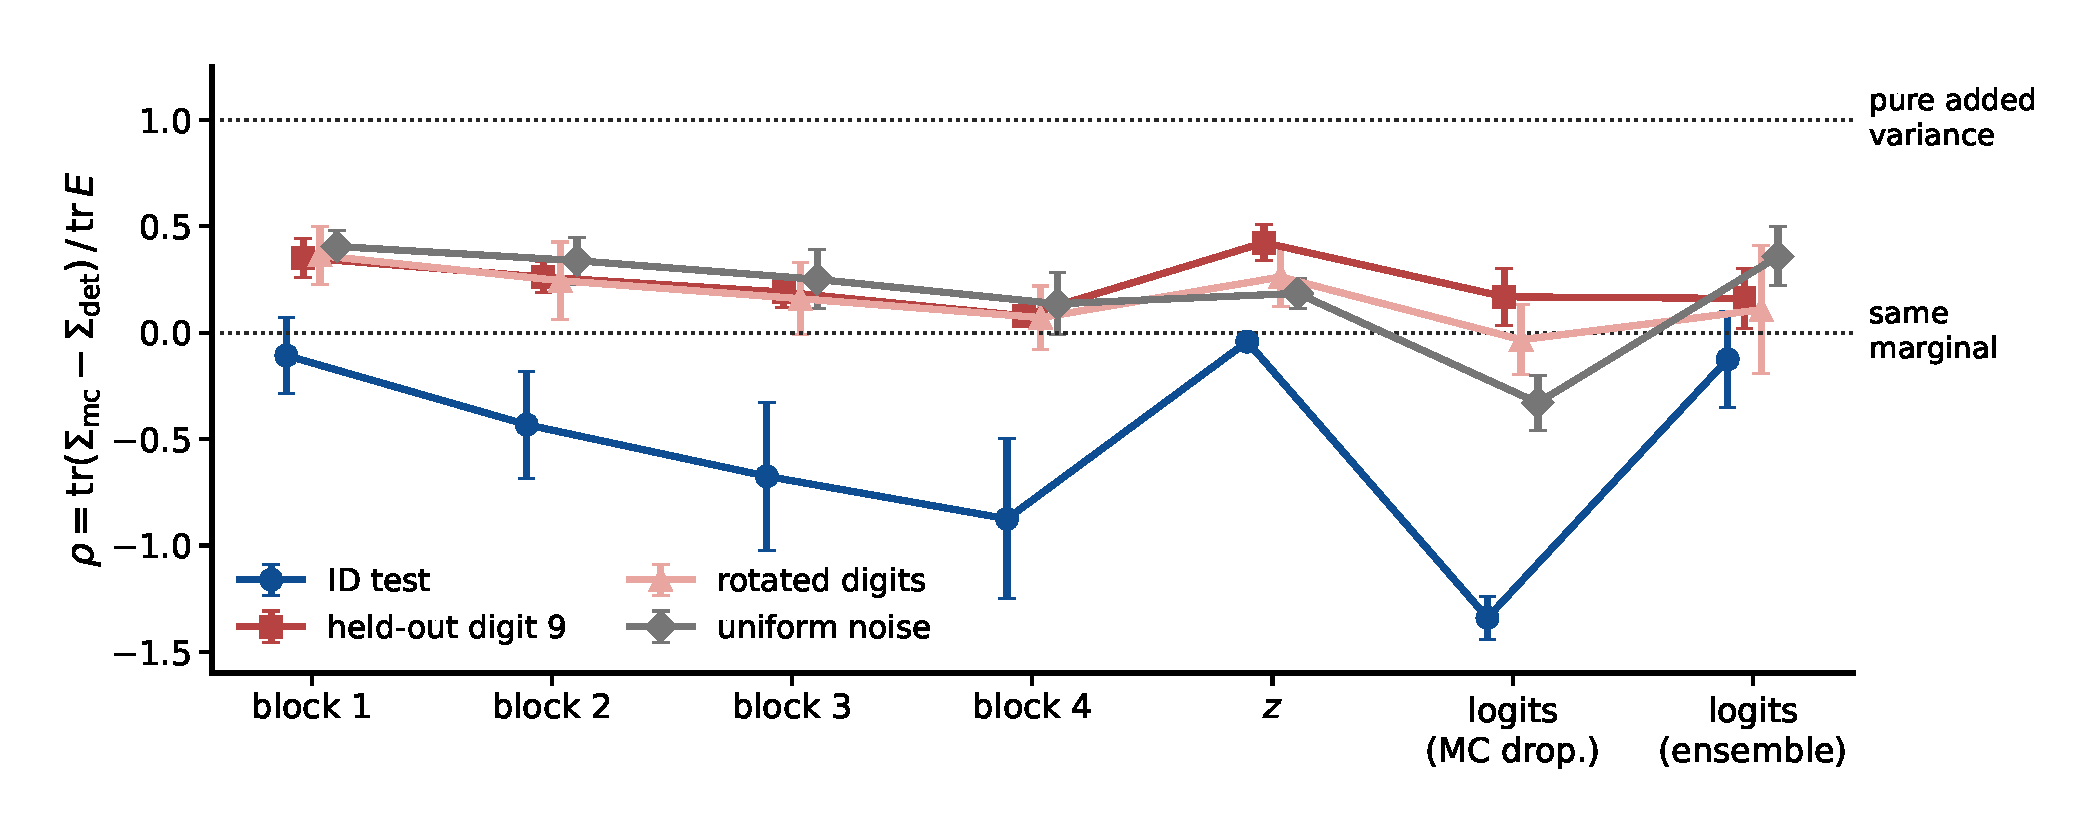
\includegraphics[width=0.86\linewidth]{fig_exp0_rho.pdf}
  \par\smallskip\raggedright\small
  \begin{itemize}
    \item In distribution at $z$, $\rho=-0.04\pm0.004$: the reference is compatible with a same-marginal flow at trace level ($7.6\%$ of the budget is per-input variance).
    \item Out of distribution at $z$, $\rho=0.19$ to $0.42$; this is allowed, because the marginal constraint binds only under $p_0$.
  \end{itemize}
\end{frame}

% ============================================================
\begin{frame}{The divergence term is required and the tree does not scale}
  \begin{columns}[c,onlytextwidth]
    \column{0.36\textwidth}
    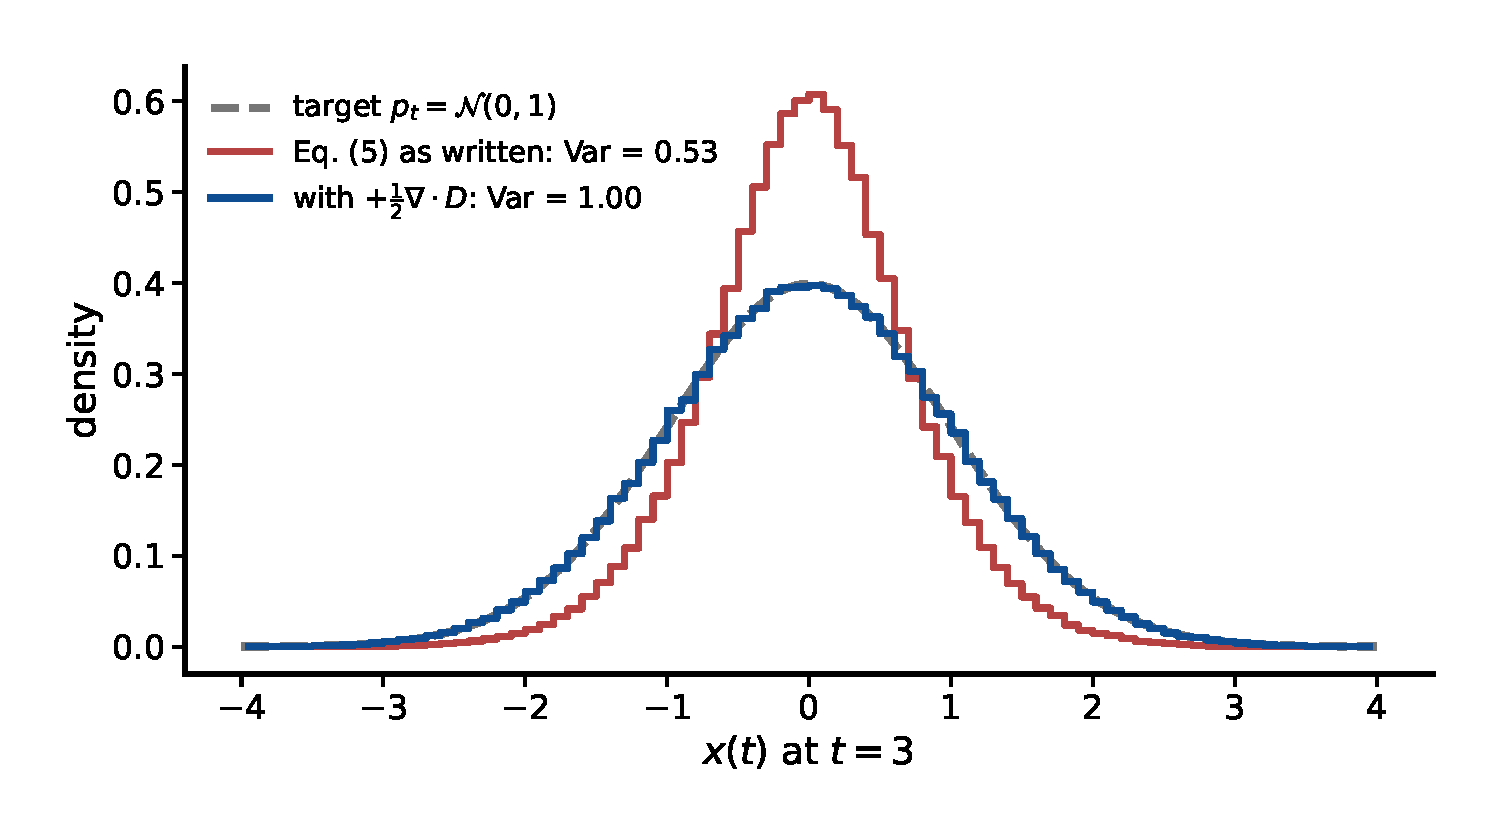
\includegraphics[width=\linewidth]{fig_drift.pdf}
    \par\footnotesize
    $g(x)=1.5\sqrt{1+x^2}$. Without $\frac12\nabla\!\cdot\!\D$: Var $0.53$ (stationary value $0.525$). With it: Var $1.00$, KS distance $0.001$.
    \column{0.61\textwidth}
    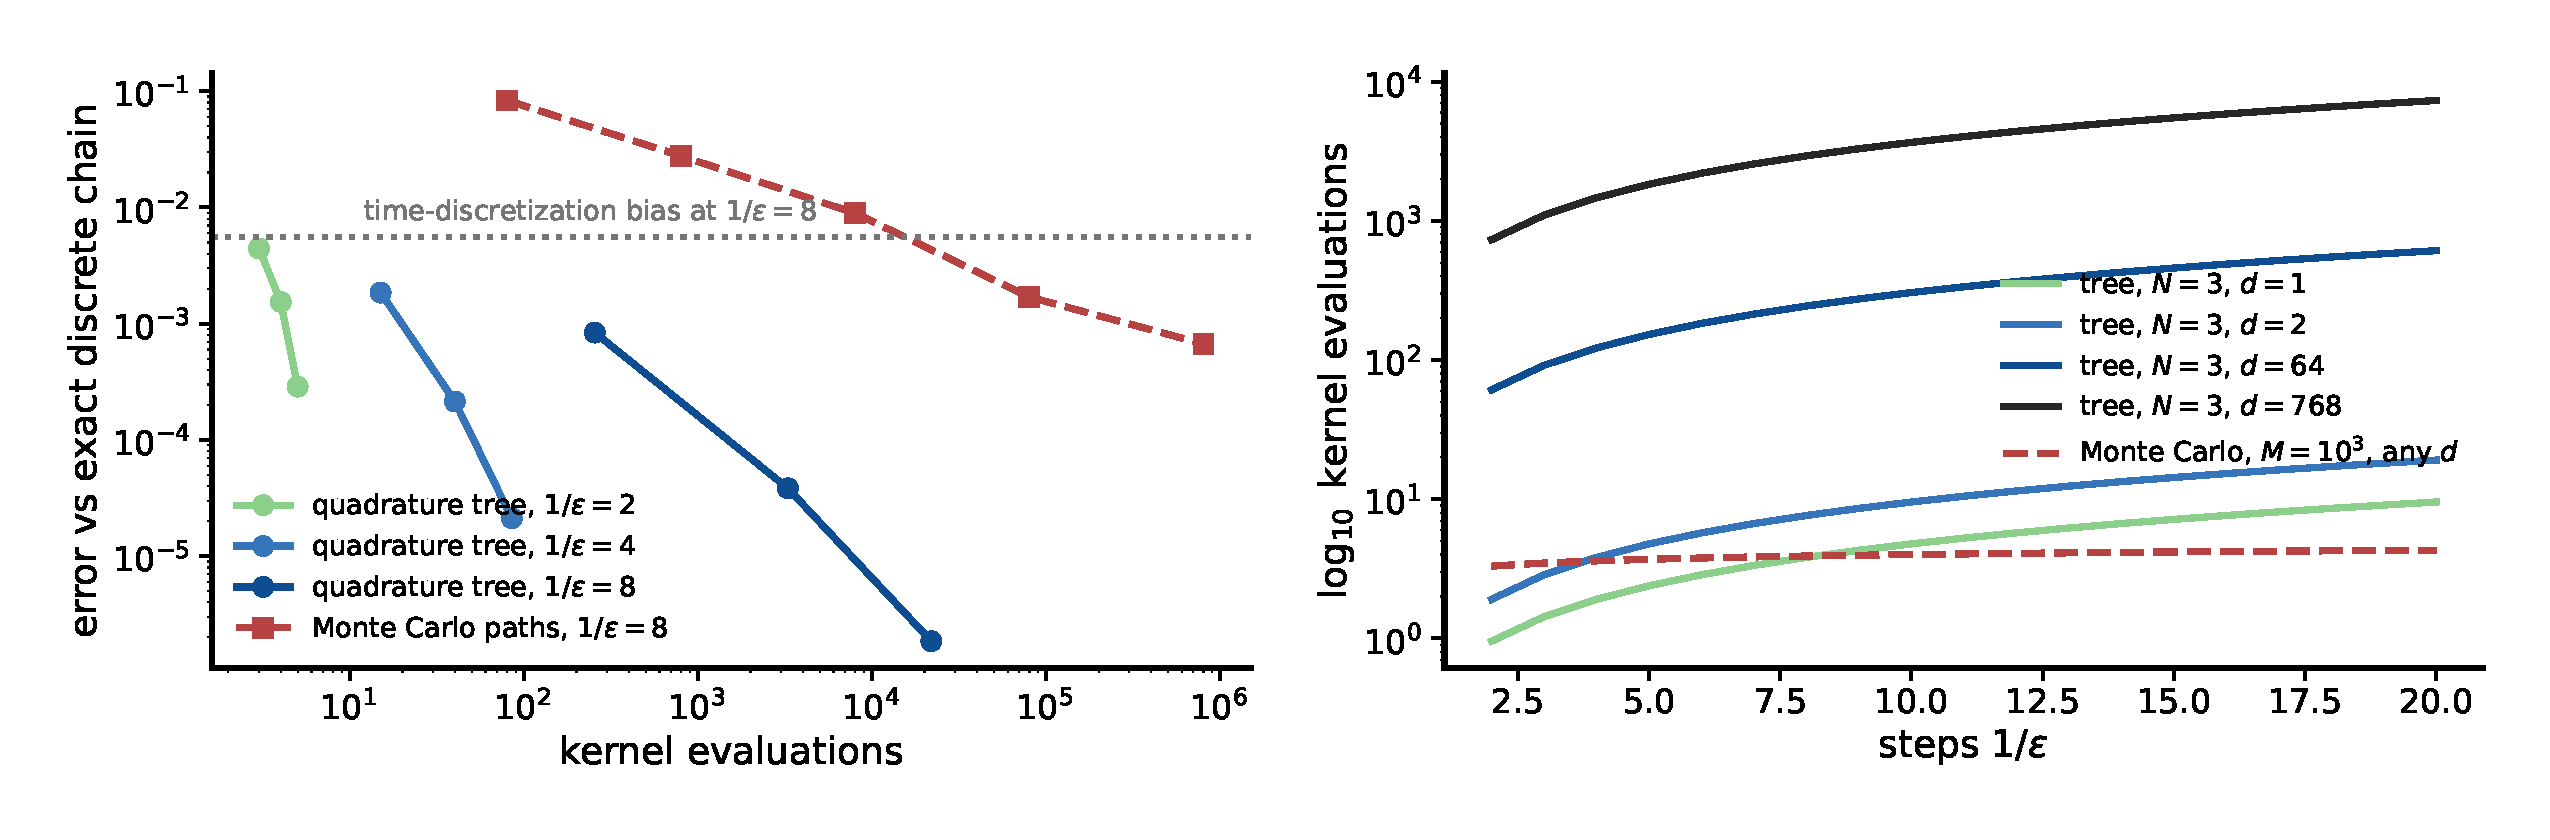
\includegraphics[width=\linewidth]{fig_cost.pdf}
    \par\footnotesize
    In 1-D the tree reaches $2\times10^{-6}$ error with $2.2\times10^{4}$ evaluations, but the cost grows as $(N^d)^{1/\epsilon}$. Both methods share the time-discretization bias ($0.0055$ at $1/\epsilon=8$).
  \end{columns}
\end{frame}

% ============================================================
\begin{frame}{The penalty of Eq.~(8) assigns variance to the wrong inputs}
  \centering
  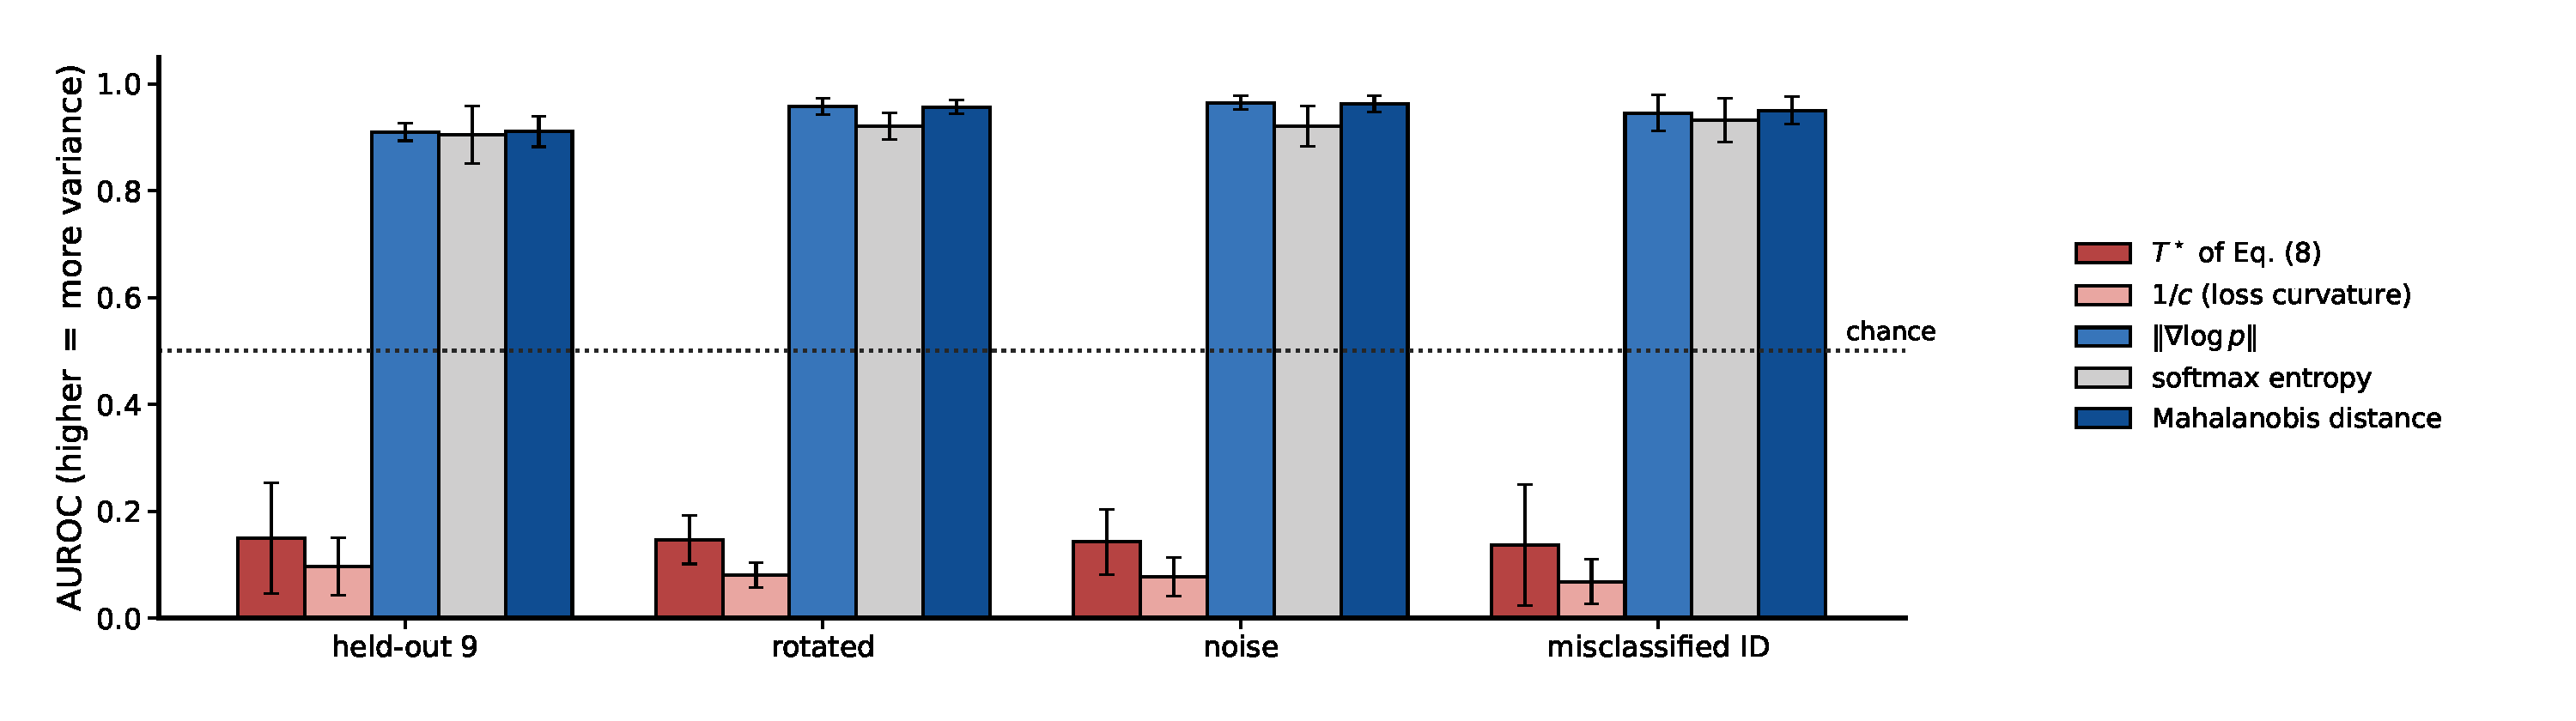
\includegraphics[width=\linewidth]{fig_eq8.pdf}
  \par\smallskip\raggedright\small
  As a detector of OOD and misclassified inputs, $T^\star$ reaches AUROC $0.14$ to $0.15$, well below chance: the curvature $c$ dominates. The score norm alone reaches $0.91$ to $0.97$, close to the Mahalanobis distance, because the score model here is Gaussian.
\end{frame}

% ============================================================
\begin{frame}{The Brownian same-marginal family does not beat simple baselines}
  \centering
  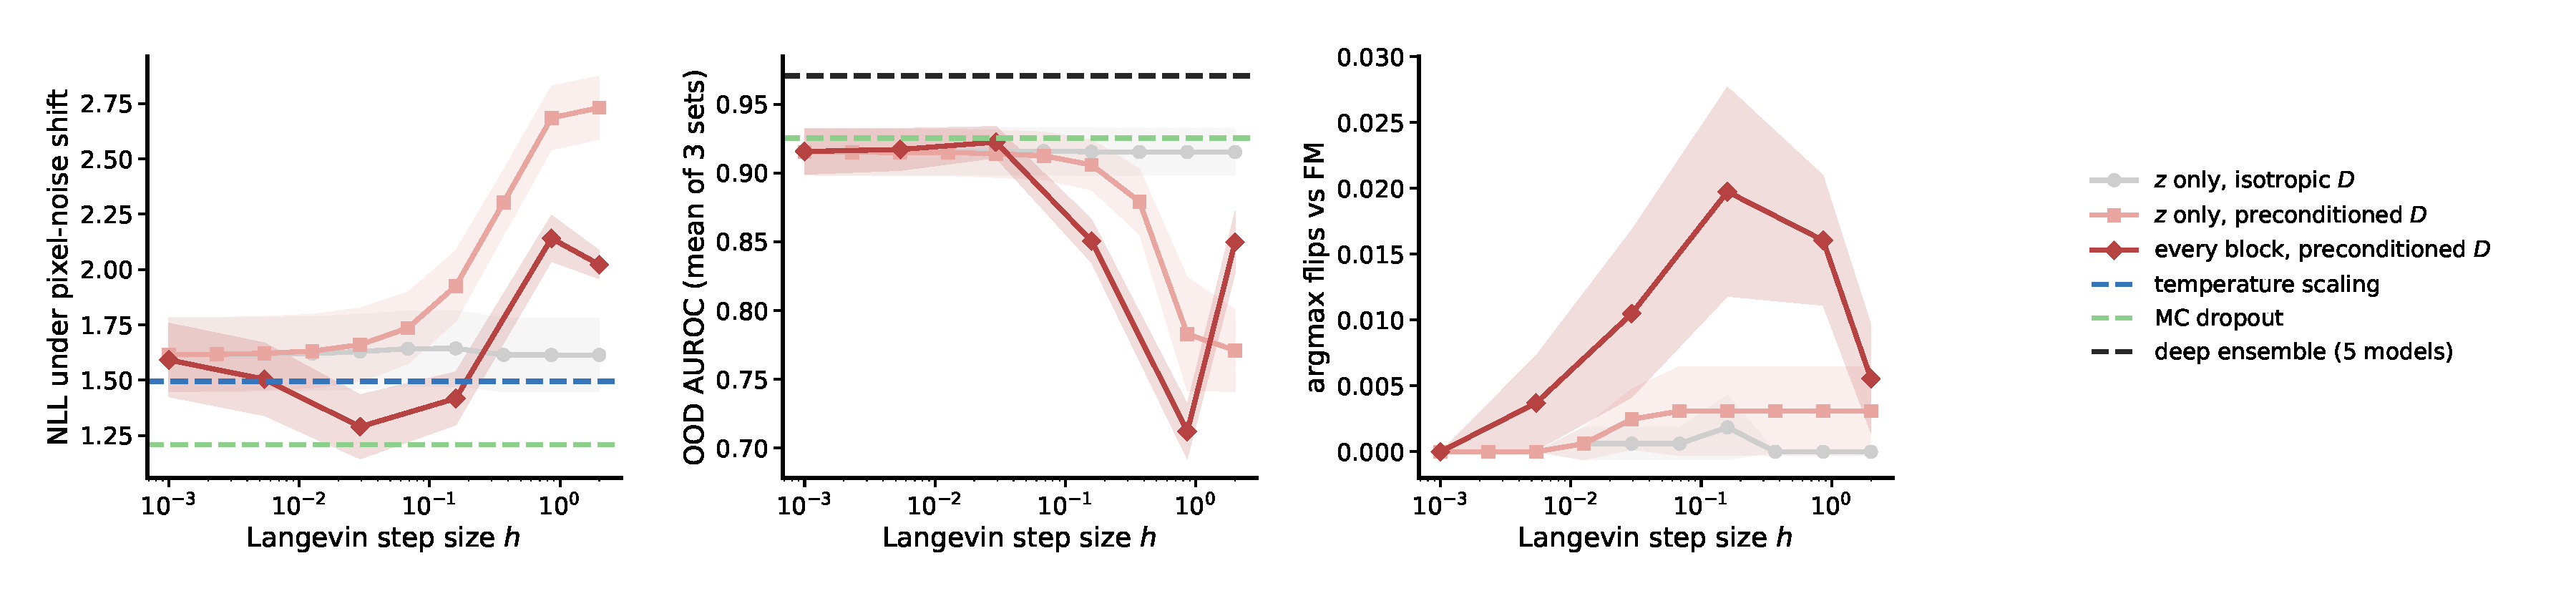
\includegraphics[width=\linewidth]{fig_brownian.pdf}
  \par\smallskip\raggedright\small
  Lie-Trotter splitting: exact FM block, then MALA targeting a class-conditional Gaussian mixture, so the family is simulated exactly. No configuration beats TS on NLL and ECE together with MC dropout on OOD AUROC, even when chosen on the test set. Larger $h$ sharpens low-margin inputs (max probability $+2.7$ points) and lowers OOD AUROC.
\end{frame}

% ============================================================
\begin{frame}{Regeneration improves calibration and OOD at no accuracy cost}
  \centering
  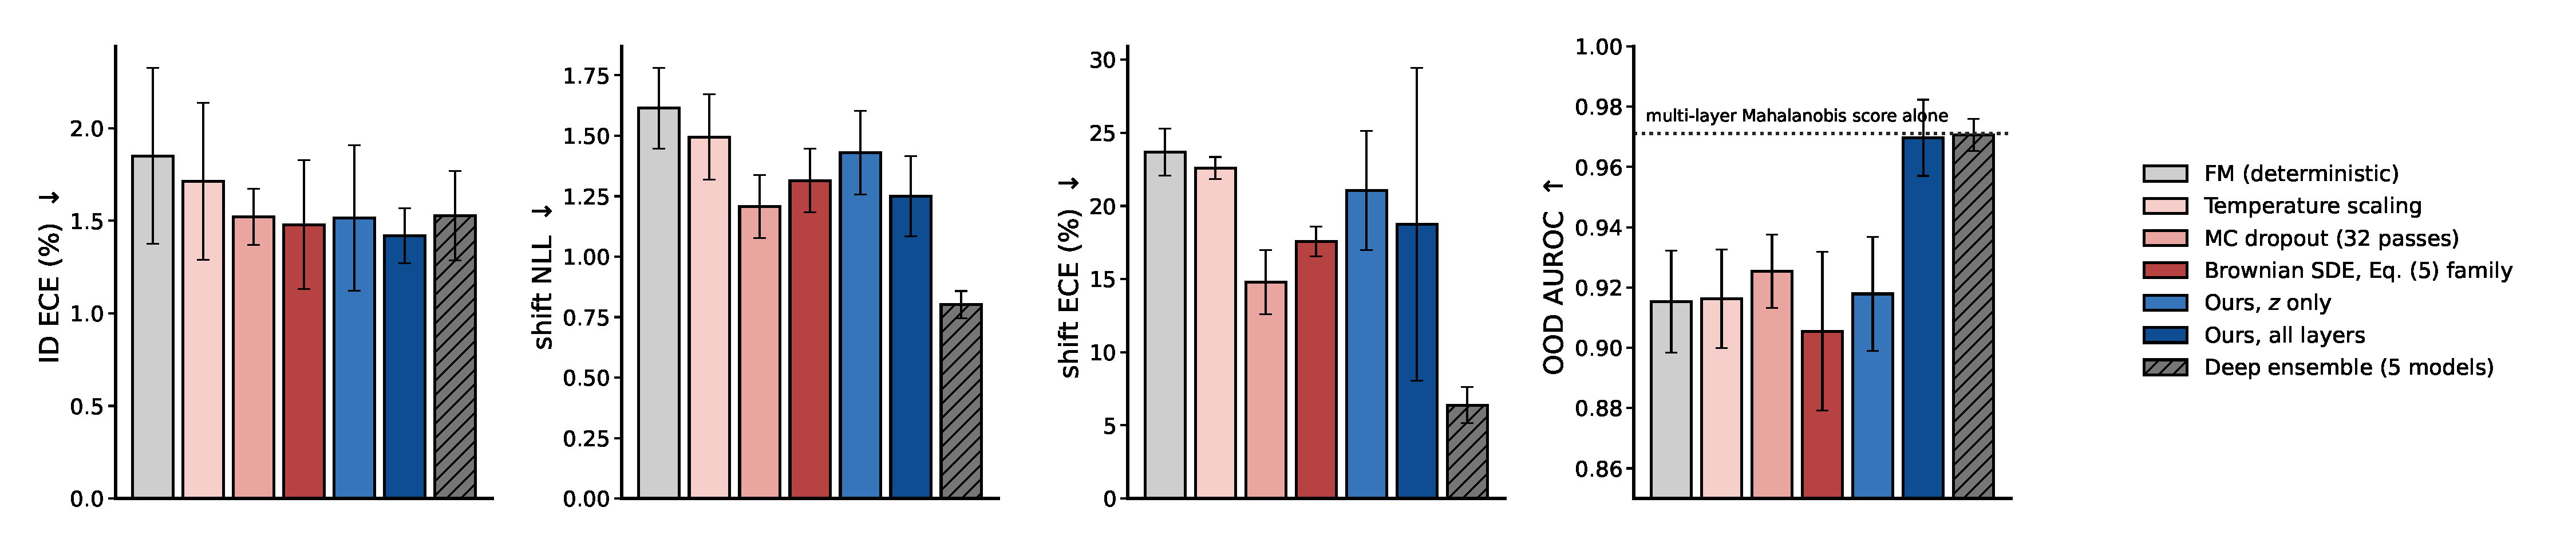
\includegraphics[width=\linewidth]{fig_main.pdf}
  \par\smallskip\raggedright\small
  \begin{itemize}
    \item Accuracy equals the FM ($97.84\%$), with no argmax flip in any split. ID ECE $1.42\pm0.15\%$, the lowest single-model value.
    \item Shift NLL $1.25\pm0.17$ (TS $1.49$, MC dropout $1.21$). OOD AUROC $0.970\pm0.013$, equal to the 5-model ensemble ($0.971$).
    \item The OOD ranking matches the multi-layer Mahalanobis score alone ($0.971$): the scaffold turns that signal into a predictive distribution. Using all layers matters ($z$ only: $0.918$).
  \end{itemize}
\end{frame}

% ============================================================
\begin{frame}{The conformal bound holds and jump mass separates far OOD}
  \centering
  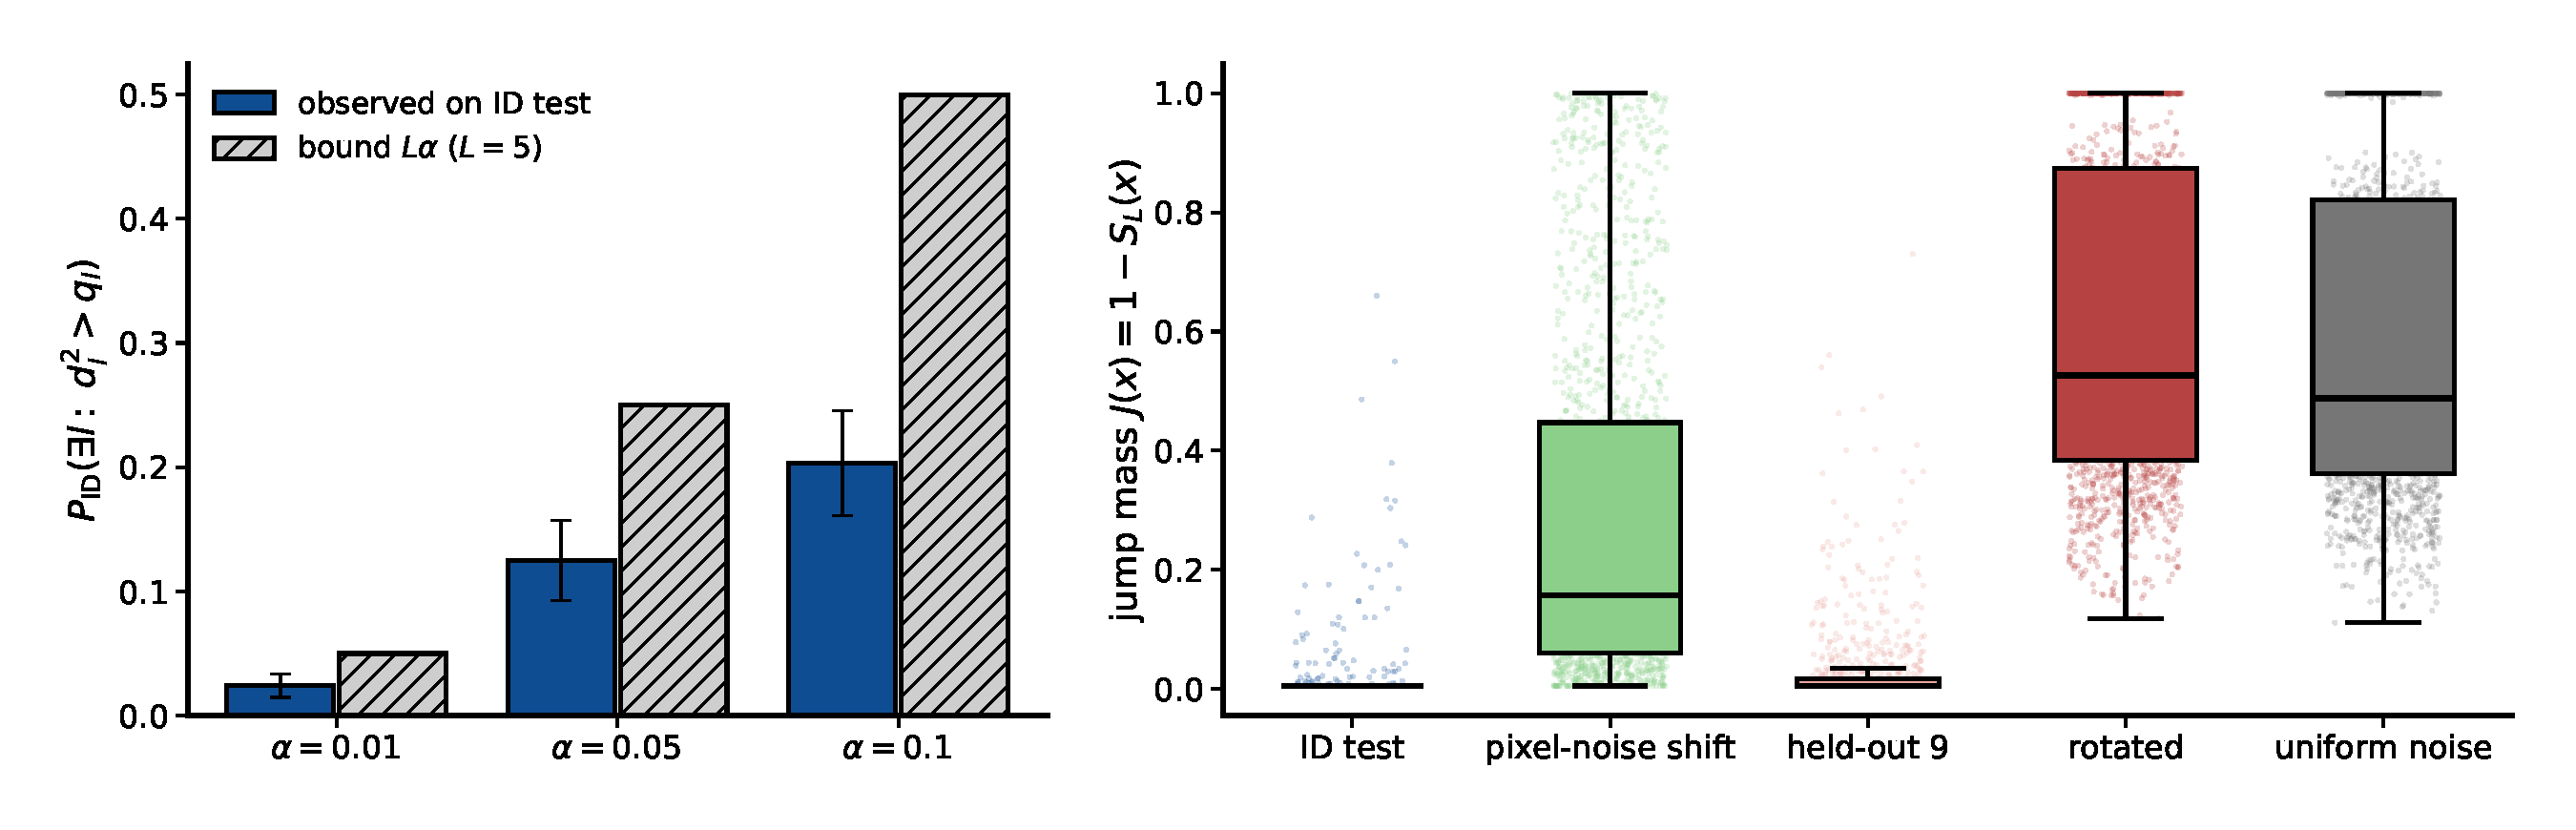
\includegraphics[width=0.94\linewidth]{fig_guarantee.pdf}
  \par\smallskip\raggedright\small
  \begin{itemize}
    \item Observed exceedance stays below $L\alpha$ for every $\alpha$ ($0.024$ vs $0.05$, $0.125$ vs $0.25$, $0.203$ vs $0.5$); the union bound is loose by about a factor of 2.
    \item Mean jump mass: ID $0.010$, shift $0.29$, rotated $0.61$, noise $0.59$, held-out 9 only $0.031$. Near OOD is the weak case.
  \end{itemize}
\end{frame}

% ============================================================
\begin{frame}{The full table shows the remaining gap to the ensemble}
  \footnotesize
  \centering
  \begin{tabular}{@{}lcccccc@{}}
    \toprule
    Method & Acc (\%) & NLL & ECE (\%) & Shift NLL & Shift ECE (\%) & OOD AUROC\\
    \midrule
    FM & 97.84 & 0.099 & 1.85 & 1.61 & 23.7 & 0.915\\
    Temperature scaling & 97.84 & 0.093 & 1.71 & 1.49 & 22.6 & 0.916\\
    MC dropout (32 passes) & 97.90 & 0.075 & 1.52 & 1.21 & 14.8 & 0.925\\
    Brownian SDE, Eq.~(5) family & 98.40 & 0.080 & 1.48 & 1.31 & 17.6 & 0.905\\
    \midrule
    Ours, $z$ only & 97.84 & 0.095 & 1.52 & 1.43 & 21.1 & 0.918\\
    Ours, all layers & 97.84 & 0.092 & \textbf{1.42} & 1.25 & 18.7 & 0.970\\
    \midrule
    Deep ensemble (5 models) & 98.95 & 0.050 & 1.53 & 0.80 & 6.4 & 0.971\\
    Multi-layer Mahalanobis (OOD only) & & & & & & 0.971\\
    \bottomrule
  \end{tabular}
  \par\medskip\raggedright
  Mean over 5 splits. Configurations of the Brownian family and of our scaffold are chosen on validation NLL only. Shift ECE of our scaffold varies across splits ($\pm10.7$), so the shift NLL is the more reliable comparison. Hoeffding certificate on Brier ($n=162$, $G=54$, $\delta=0.05$): slack $0.31$, valid but loose at this sample size.
\end{frame}

% ============================================================
\section{ImageNet ladder (ViT-B/16)}

\begin{frame}{The ImageNet ladder separates compilation error from the uncertainty layer}
  \small
  \begin{itemize}
    \item \textbf{FM.} ViT-B/16 (in21k, fine-tuned on in1k; the HuggingFace checkpoint used by DIRECTOR). Top-1 $81.7\%$, ReaL $86.7\%$.
    \item \textbf{Data.} ImageNet-1k validation split into calA (5k, conformal thresholds), calB (5k, selection and temperature) and test (40k). Regeneration pool and compile data: 100k train images (about 100 per class). Shift: ImageNet-C definitions at severity 3 (Gaussian noise, blur, contrast, JPEG; 20k). OOD: ImageNet-O, DTD textures, uniform noise.
    \item \textbf{Rungs.} (1) FM; (2) compiled flow $\Ft$ by Eq.~(7) with a rollout term, for the last 4 blocks and for all 12; (3) Brownian same-marginal SDE at $z$ (MALA, 1000-class GMM); (4) regeneration scaffold, population and partitioned. Rungs 3 and 4 run on the FM and on the compiled flow.
    \item \textbf{Baselines.} Temperature scaling, test-time dropout injection (8 passes), a 3-checkpoint ensemble, the multi-layer Mahalanobis score.
  \end{itemize}
  \source{Code: uq/imagenet\_ladder. Selection uses calB only; every number below is on the 40k test split, the shift set or the OOD sets.}
\end{frame}

% ============================================================
\begin{frame}{Compiling even the last four blocks loses a third of the FM predictions}
  \centering
  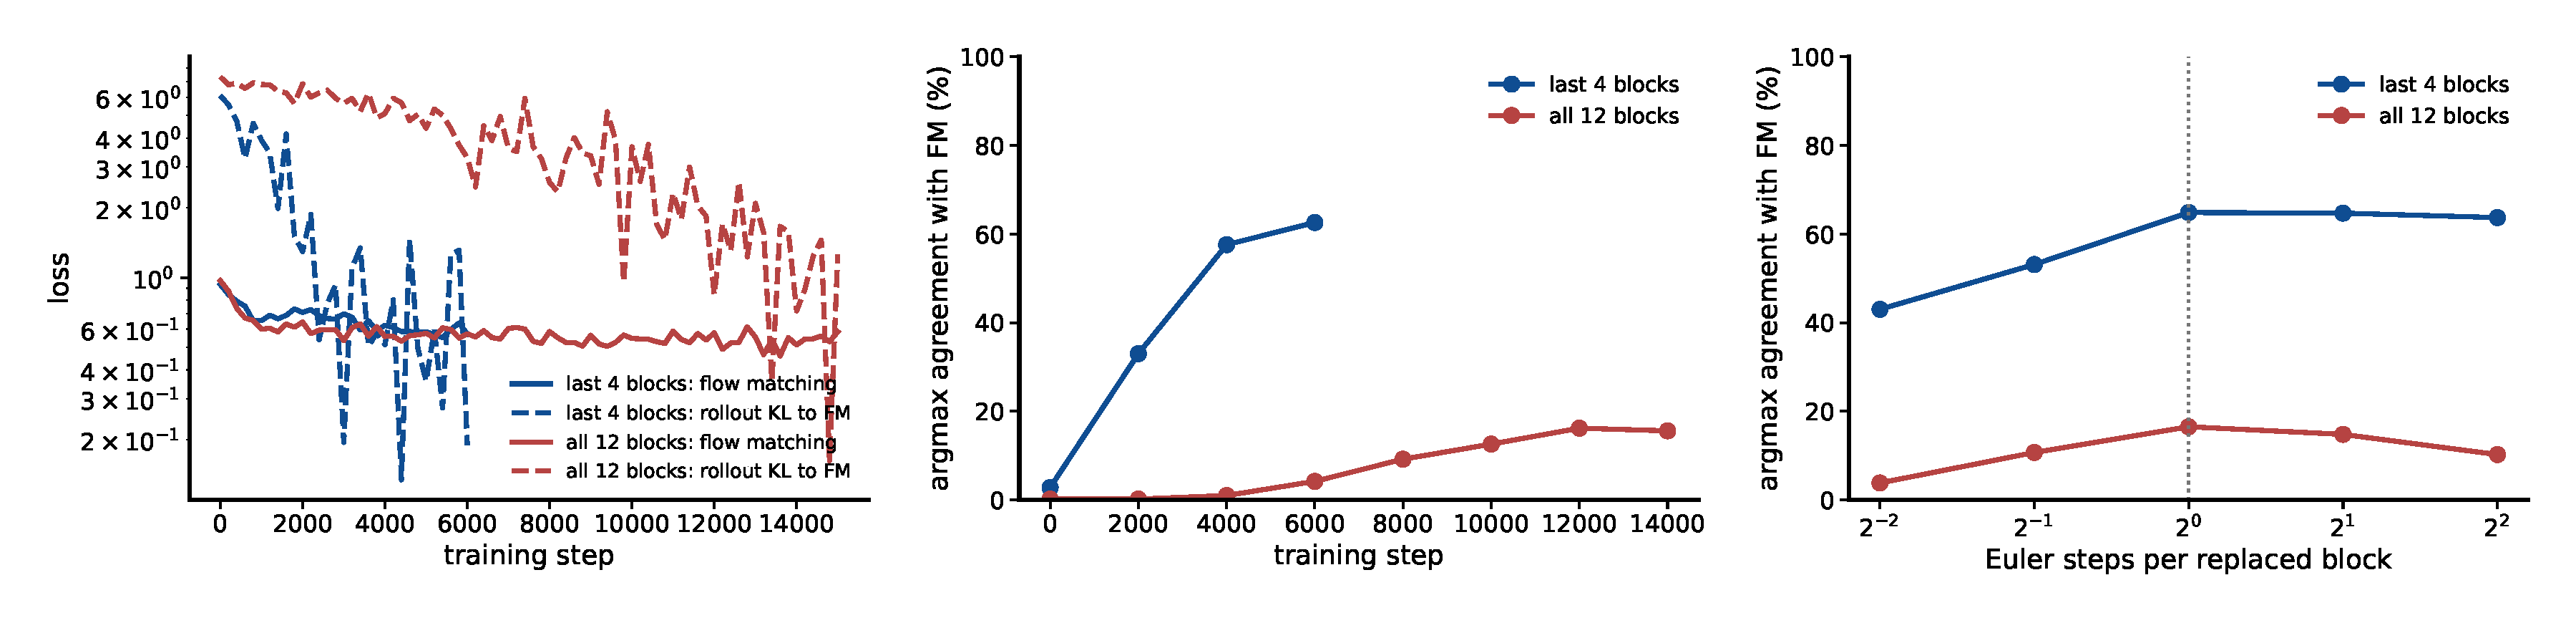
\includegraphics[width=\linewidth]{fig_in_compile.pdf}
  \par\smallskip\raggedright\small
  \begin{itemize}
    \item Last 4 blocks, 6000 steps: argmax agreement with the FM $64.1\%$ on test, top-1 $60.6\%$ (FM $81.7\%$), ECE $11.2\%$. All 12 blocks, 15000 steps: agreement $16.3\%$, top-1 $15.8\%$, NLL $4.30$, OOD AUROC $0.46$.
    \item More Euler steps do not help beyond one per replaced block (last 4: $64.9$, $64.7$, $63.7\%$; all 12: $16.5$, $14.8$, $10.2\%$ at 1, 2, 4 steps per block): the learned field is not a convergent ODE, so the $\epsilon$ knob of Eq.~(6) has nothing to converge to.
  \end{itemize}
\end{frame}

% ============================================================
\begin{frame}{More data helps the compiled flow, per-block adapters do not}
  \centering
  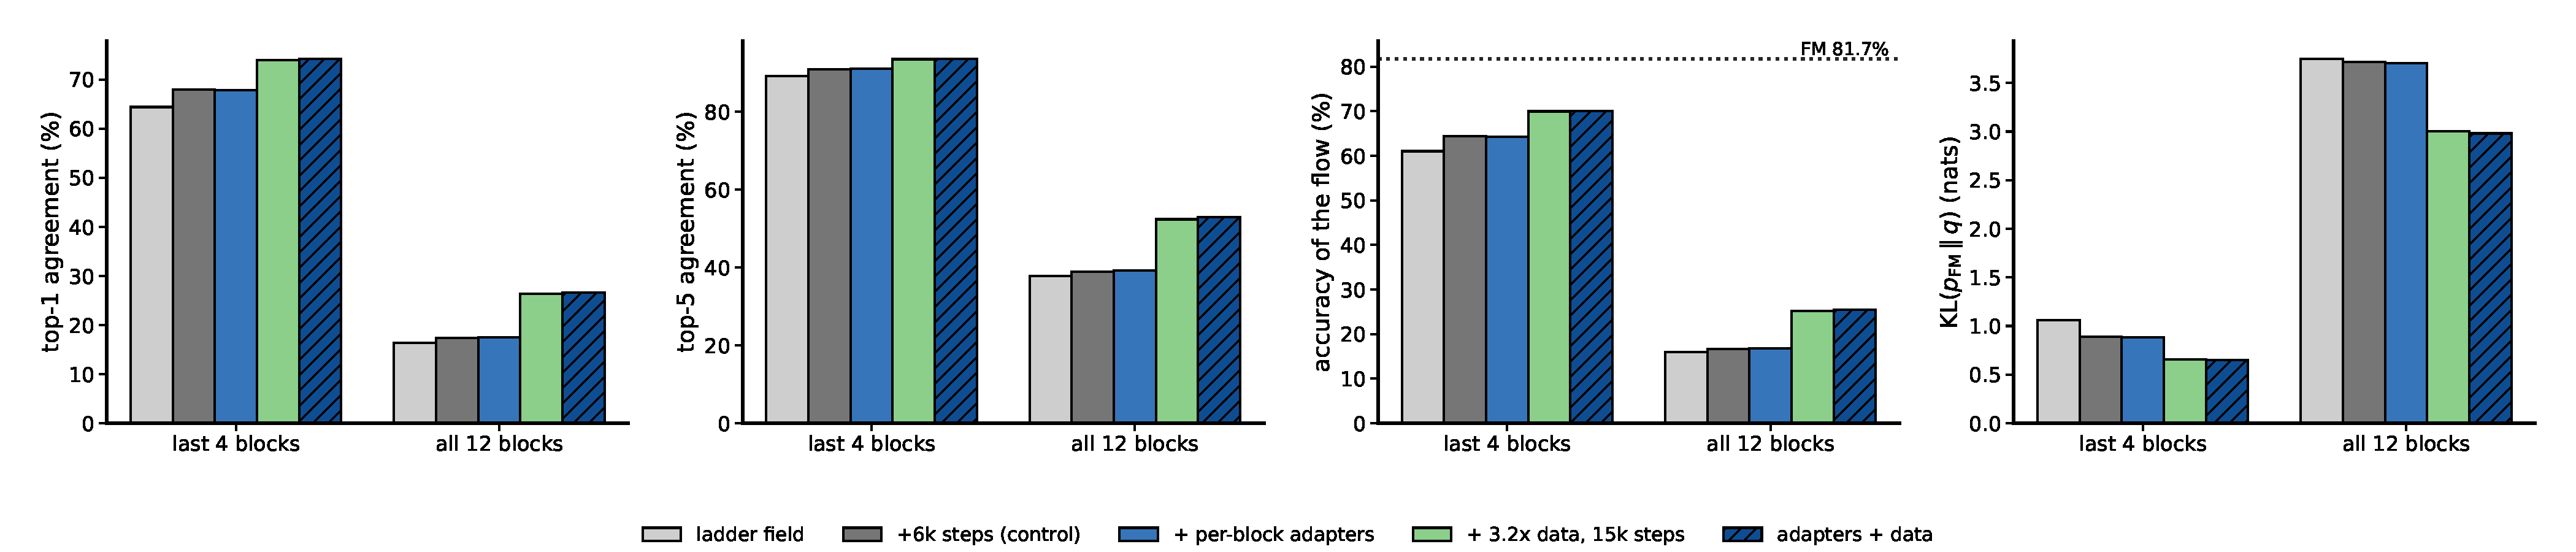
\includegraphics[width=\linewidth]{fig_in_fidelity_options.pdf}
  \par\smallskip\raggedright\small
  \begin{itemize}
    \item Every arm continues from the ladder field; scores on 10k test images. Per-block rank-32 adapters ($+28$M parameters) change top-1 agreement by at most $0.3$ points.
    \item $3.2\times$ more images and $15$k more steps: last 4 blocks $64.4\to74.0\%$ top-1, $93.5\%$ top-5, KL $1.06\to0.66$, accuracy $61.0\to70.0\%$ (FM $81.7\%$); all 12 blocks $16.4\to26.4\%$.
    \item The compiled flow is data limited, and still far from the FM: claims about uncertainty on a compiled ImageNet flow must wait for a field that reaches high fidelity.
  \end{itemize}
\end{frame}

% ============================================================
\begin{frame}{At 1000 classes the scaffolds keep their guarantees but lose their gains}
  \centering
  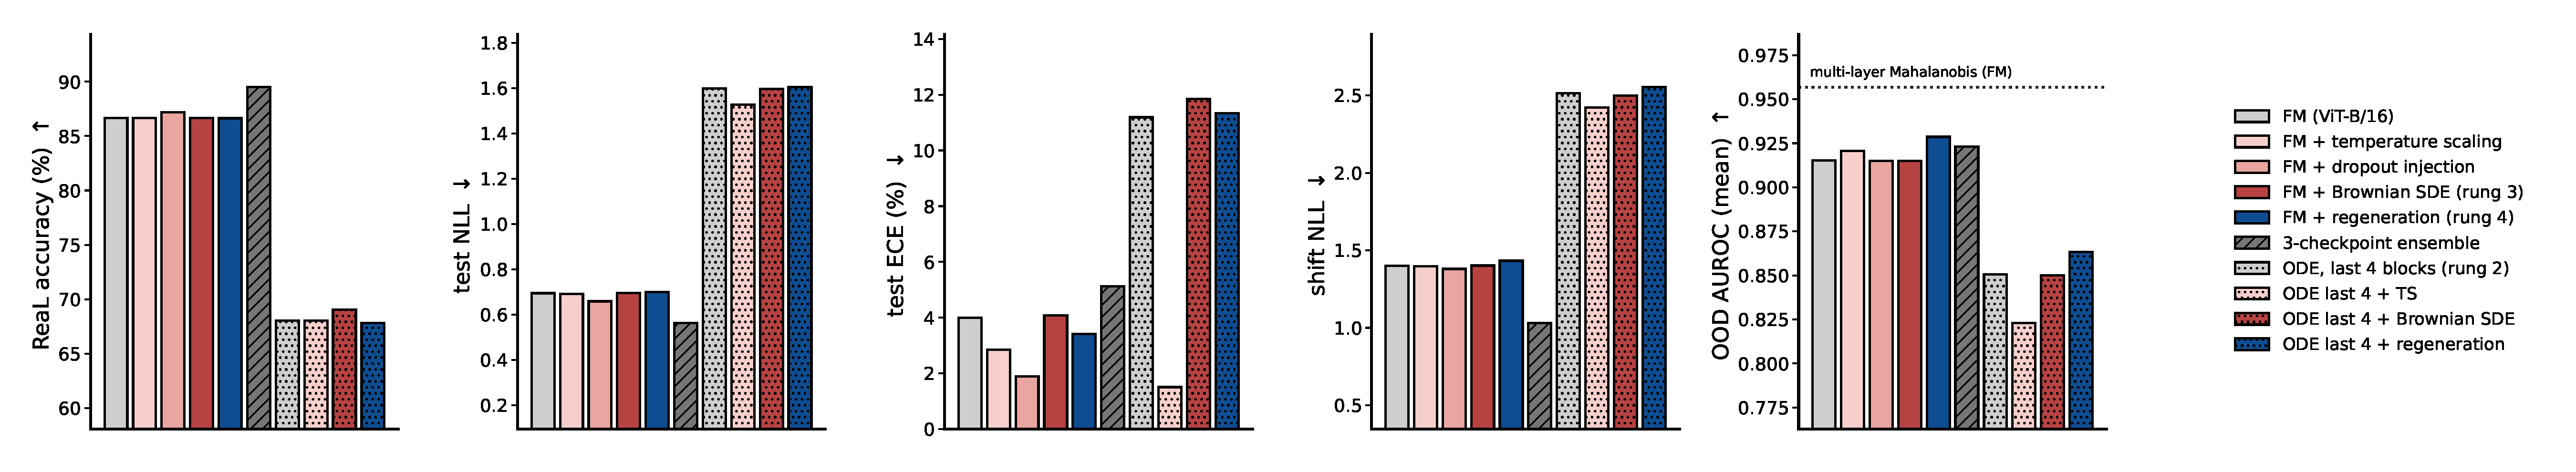
\includegraphics[width=\linewidth]{fig_in_ladder.pdf}
  \par\smallskip\raggedright\small
  \begin{itemize}
    \item Conformal bound holds: ID exceedance $0.034\le L\alpha=0.06$; flips $0.27\%$, of which $0.07\%$ turn a correct ReaL label wrong.
    \item Population regeneration raises NLL ($0.695\to0.700$) and shift NLL ($1.401\to1.432$); selection on calB picks the gentlest setting. The Brownian family at $z$ is a no-op once selected ($h=0.003$).
    \item On the compiled flow, temperature scaling repairs the overconfidence (ECE $11.2\to1.5\%$); the scaffolds do not.
  \end{itemize}
\end{frame}

% ============================================================
\begin{frame}{Partitioned regeneration removes the NLL cost but not the OOD gap}
  \footnotesize
  \centering
  \begin{tabular}{@{}lcccccc@{}}
    \toprule
    Method on the FM & ReaL (\%) & NLL & ECE (\%) & Shift NLL & Shift ECE (\%) & OOD AUROC\\
    \midrule
    FM & 86.65 & 0.695 & 4.00 & 1.401 & 6.3 & 0.915\\
    Temperature scaling & 86.65 & 0.692 & 2.84 & 1.397 & 4.5 & 0.921\\
    Brownian SDE at $z$ (rung 3) & 86.67 & 0.695 & 4.08 & 1.402 & 6.4 & 0.915\\
    Population regeneration (rung 4) & 86.64 & 0.700 & 3.41 & 1.432 & 3.7 & 0.929\\
    Partitioned regeneration, $\tau=1$ & 86.64 & 0.691 & 3.30 & 1.393 & 5.5 & 0.918\\
    \midrule
    Dropout injection (8 passes) & 87.20 & \textbf{0.658} & \textbf{1.90} & 1.380 & \textbf{3.0} & 0.915\\
    3-checkpoint ensemble & \textbf{89.49} & 0.563 & 5.12 & \textbf{1.031} & 10.8 & 0.923\\
    Multi-layer Mahalanobis (OOD only) & & & & & & \textbf{0.957}\\
    \bottomrule
  \end{tabular}
  \par\medskip\raggedright\small
  \begin{itemize}
    \item As derived, reverting toward the predicted class ($\tau=1$) removes the NLL cost: NLL $0.691$, below the FM and TS. It also adds less entropy off the data, so OOD AUROC falls to $0.918$.
    \item The distance signal is strong ($0.957$) but neither scaffold turns it into a predictive that ranks OOD as well.
  \end{itemize}
\end{frame}

% ============================================================
\begin{frame}{Corruption and OOD breakdowns locate the remaining gaps}
  \centering
  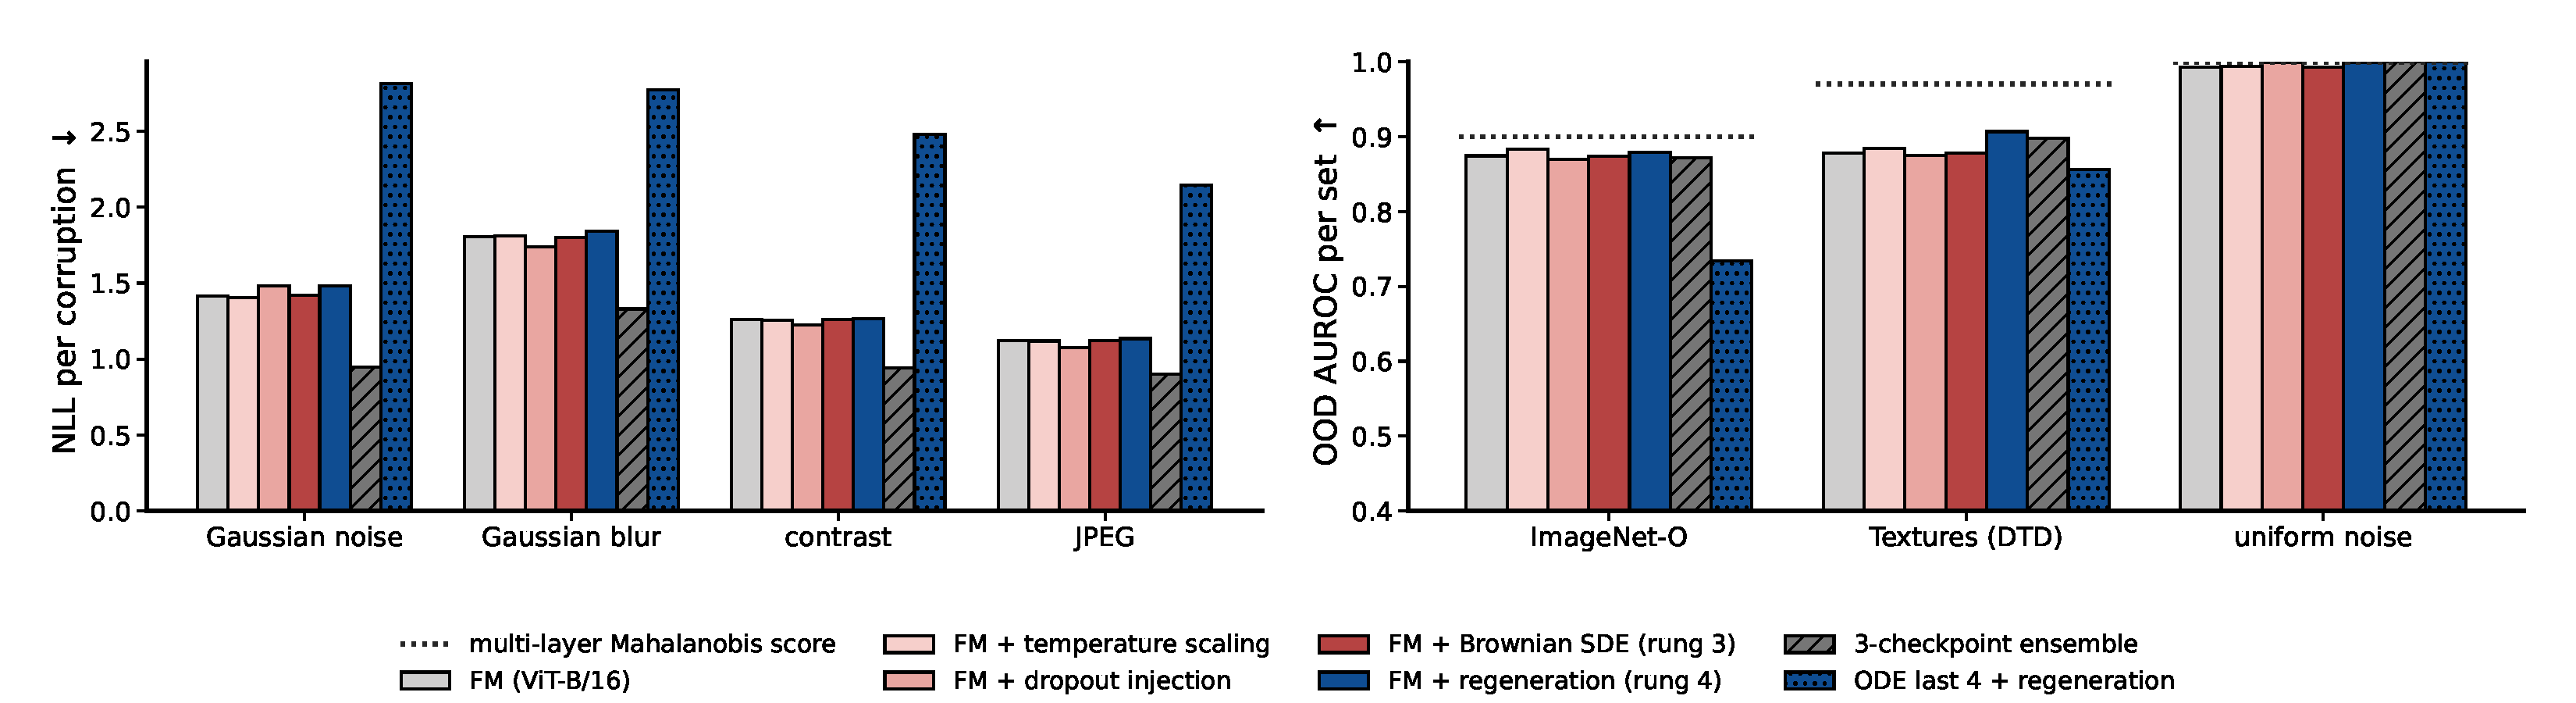
\includegraphics[width=\linewidth]{fig_in_breakdown.pdf}
  \par\smallskip\raggedright\small
  The ensemble dominates every corruption type. Regeneration helps only on Textures (AUROC $0.879\to0.907$), where the distance score alone reaches $0.970$. On ImageNet-O every predictive stays below $0.89$; the distance score reaches $0.900$.
\end{frame}

% ============================================================
\section{CIFAR ladder (DIRECTOR setting)}

\begin{frame}{The CIFAR ladder repeats the DIRECTOR setting with a calibrated fine-tune}
  \small
  \begin{itemize}
    \item \textbf{FM.} The same ViT-B/16 checkpoint as DIRECTOR (Appendix A.6.1), fine-tuned 3 epochs at 224 px without label smoothing. Split: 45k fine-tune, 5k held out (calA 2.5k, calB 2.5k), official 10k test.
    \item \textbf{Shift.} CIFAR-10-C and CIFAR-100-C: all 15 corruptions and 5 severities, 400 test images per cell. \textbf{OOD.} SVHN, the other CIFAR, LSUN (resize), Textures, noise.
  \end{itemize}
  \medskip
  \centering
  \begin{tabular}{@{}lcccc@{}}
    \toprule
    ViT-B/16 on CIFAR-10 & Acc (\%) & ECE (\%) & NLL & Brier\\
    \midrule
    DIRECTOR baseline (Table 6) & 97.88 & 18.02 & 0.256 & 0.068\\
    DIRECTOR reconfiguration (Table 6) & 97.17 & 1.61 & 0.112 & 0.048\\
    Our fine-tuned FM & \textbf{98.79} & \textbf{0.63} & \textbf{0.044} & \textbf{0.020}\\
    \bottomrule
  \end{tabular}
  \par\medskip\raggedright\small
  The large ECE of the DIRECTOR baseline comes from its fine-tuning recipe, not from ViT-B: a plain fine-tune is already calibrated, so CIFAR leaves little ID calibration to gain.
\end{frame}

% ============================================================
\begin{frame}{On CIFAR the scaffold beats both the softmax and the distance score on OOD}
  \centering
  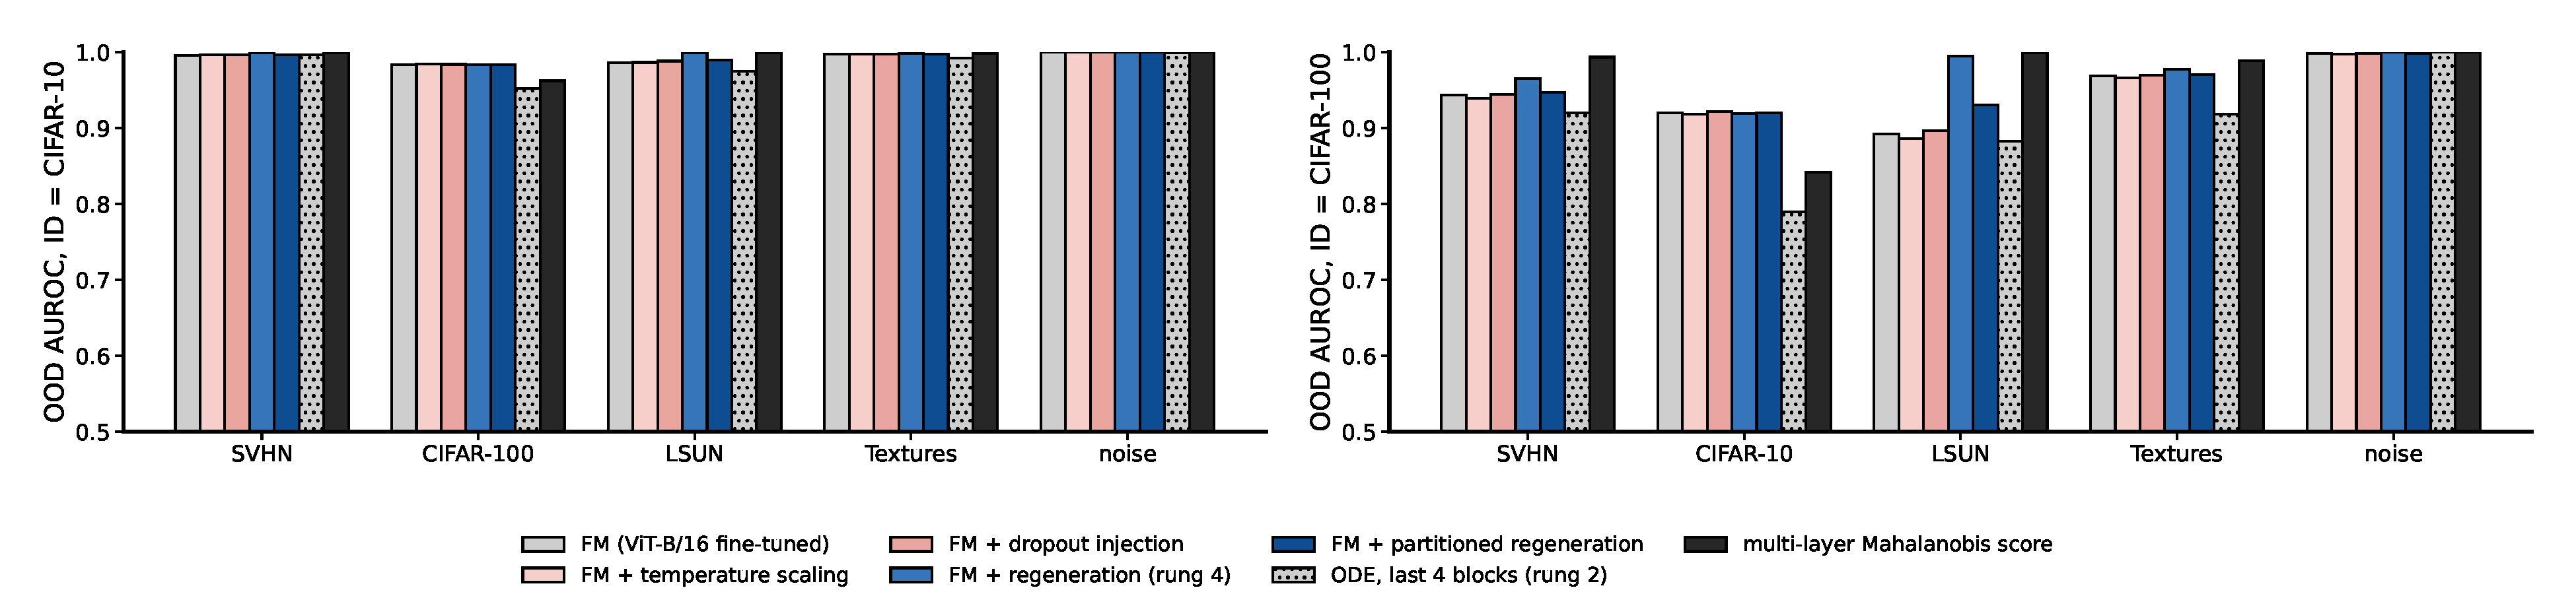
\includegraphics[width=\linewidth]{fig_cifar_ood.pdf}
  \par\smallskip\raggedright\small
  \begin{itemize}
    \item CIFAR-100: mean OOD AUROC $0.972$ (FM $0.945$, distance score alone $0.965$); LSUN $0.892\to0.995$, SVHN $0.944\to0.966$. CIFAR-10: $0.996$ (FM $0.993$, distance $0.992$).
    \item The distance score fails on near OOD (CIFAR-10 vs CIFAR-100: $0.842$); the scaffold keeps the softmax level there ($0.920$), so it combines the two signals. This did not happen on ImageNet.
  \end{itemize}
\end{frame}

% ============================================================
\begin{frame}{The OOD gain costs NLL, and the partitioned target trades it back}
  \footnotesize
  \centering
  \begin{tabular}{@{}lcccccc@{}}
    \toprule
    & \multicolumn{3}{c}{CIFAR-10} & \multicolumn{3}{c}{CIFAR-100}\\
    \cmidrule(lr){2-4}\cmidrule(lr){5-7}
    Method on the FM & NLL & C-NLL & OOD & NLL & C-NLL & OOD\\
    \midrule
    FM & 0.044 & 0.312 & 0.993 & 0.265 & 1.017 & 0.945\\
    Temperature scaling & 0.043 & \textbf{0.297} & 0.993 & \textbf{0.262} & 1.042 & 0.942\\
    Dropout injection (8 passes) & \textbf{0.040} & 0.311 & 0.993 & 0.263 & 1.023 & 0.946\\
    Brownian SDE at $z$ & 0.045 & 0.313 & 0.993 & 0.265 & 1.019 & 0.945\\
    Population regeneration & 0.049 & 0.374 & \textbf{0.996} & 0.271 & 1.092 & \textbf{0.972}\\
    Partitioned regeneration, $\tau=1$ & 0.044 & 0.308 & 0.994 & 0.265 & \textbf{1.016} & 0.953\\
    Multi-layer Mahalanobis (OOD only) & & & 0.992 & & & 0.965\\
    \bottomrule
  \end{tabular}
  \par\medskip\raggedright\small
  \begin{itemize}
    \item The trade-off follows $q_y-p_y=J(m_y-p_y)$: reverting to the population predictive helps OOD and costs NLL whenever the FM is right; reverting within the predicted class removes the cost and keeps part of the gain.
    \item Guarantees hold on both datasets: ID exceedance $0.028$ and $0.032\le L\alpha=0.06$; flips $0.00\%$ and $0.05\%$.
  \end{itemize}
\end{frame}

% ============================================================
\begin{frame}{Calibration under corruption degrades similarly for every method}
  \centering
  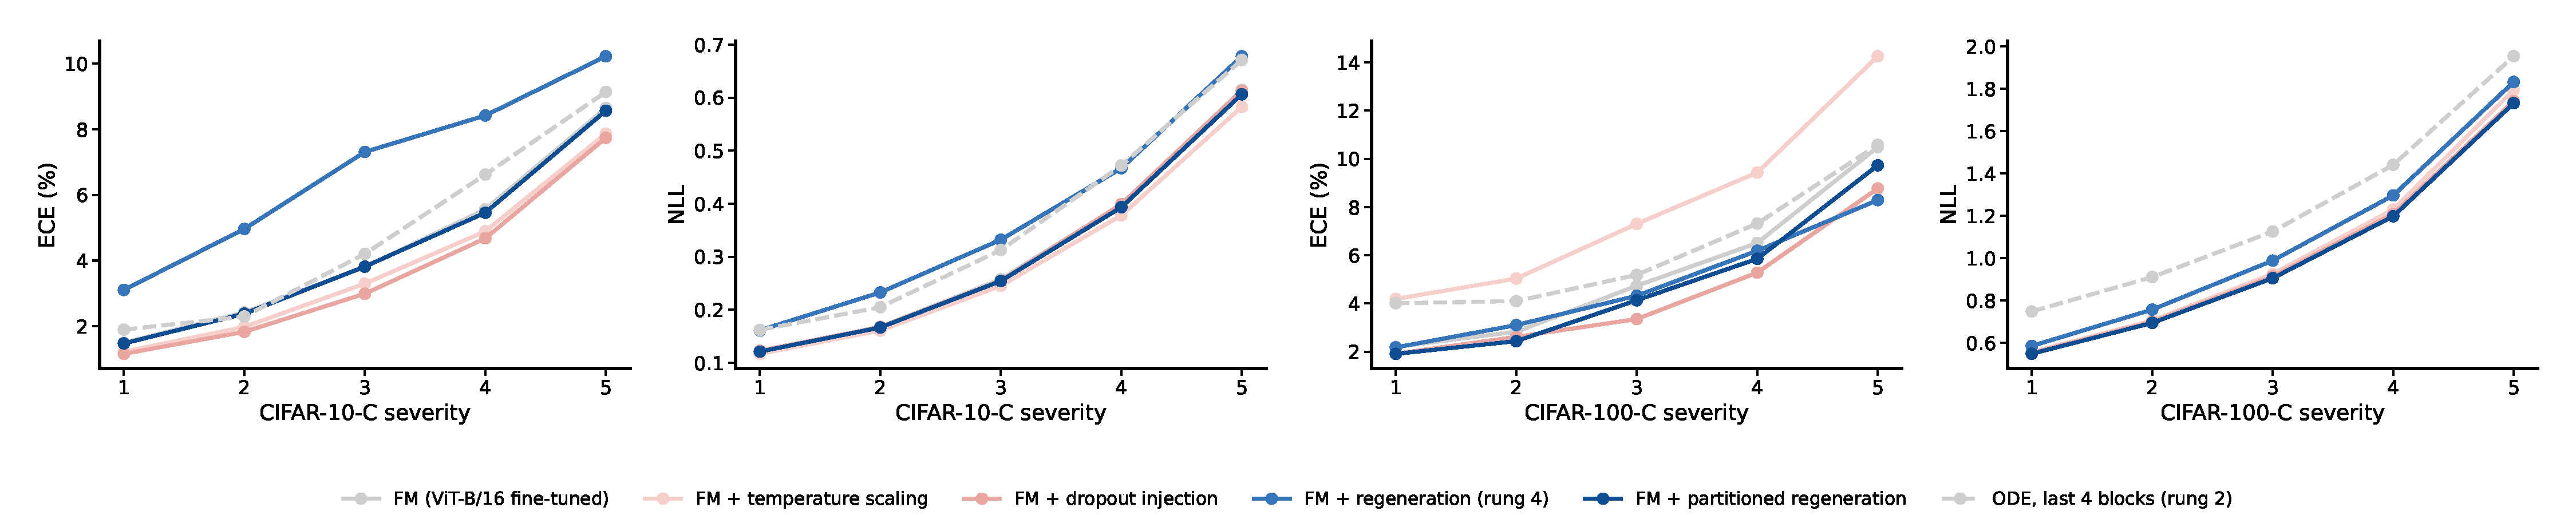
\includegraphics[width=\linewidth]{fig_cifar_severity.pdf}
  \par\smallskip\raggedright\small
  ECE and NLL on CIFAR-C rise with severity for all methods. Population regeneration has the highest ECE on CIFAR-10-C at every severity and the lowest on CIFAR-100-C at severity 5 ($8.3\%$ vs FM $10.5\%$). Dropout injection has the lowest ECE at most other severities.
\end{frame}

% ============================================================
\begin{frame}{Compilation fidelity falls with the number of classes and of compiled blocks}
  \centering
  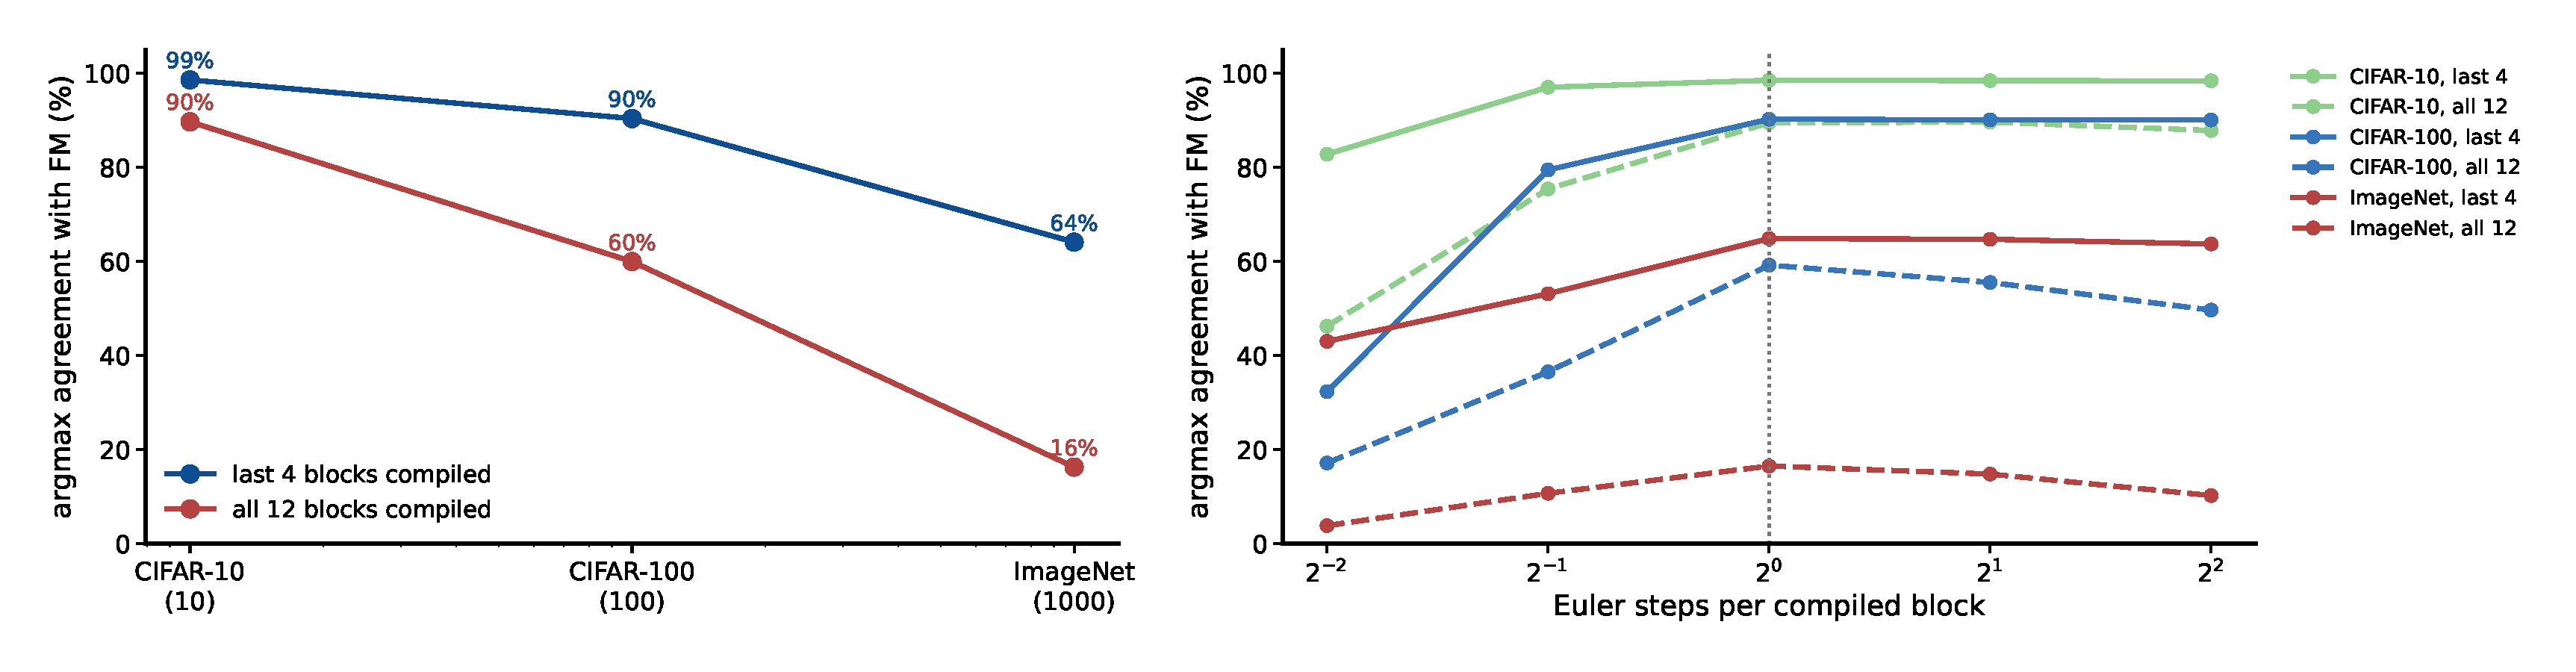
\includegraphics[width=\linewidth]{fig_compile_scaling.pdf}
  \par\smallskip\raggedright\small
  \begin{itemize}
    \item Argmax agreement with the FM, last 4 / all 12 blocks: CIFAR-10 $98.6/89.7\%$, CIFAR-100 $90.4/60.0\%$, ImageNet $64.1/16.3\%$. Top-1 of the 12-block flow: $89.4\%$ (CIFAR-10), $59.1\%$ (CIFAR-100), $15.8\%$ (ImageNet).
    \item In all six compiles agreement stops improving at one Euler step per block (at most $+0.1$ point beyond it): the field is a per-block map, not a convergent ODE, so the $\epsilon$ control of Eq.~(6) has no limit to approach.
  \end{itemize}
\end{frame}

% ============================================================
\begin{frame}{Three findings define the next experiments}
  \small
  \begin{enumerate}
    \item \textbf{Compilation is the bottleneck.} One shared field keeps $98.6\%$ of the FM predictions on CIFAR-10 (last 4 blocks) but only $16.3\%$ on ImageNet (all 12). Per-block adapters do not help; $3.2\times$ more data does ($64\to74\%$). Next: the full training set, and fidelity reported before any uncertainty number.
    \item \textbf{The reversion target sets the trade-off.} By $q_y-p_y=J(m_y-p_y)$, the population target buys OOD AUROC (CIFAR-100: $0.945\to0.972$) at an NLL cost that grows with $C$; the partitioned target removes the cost and keeps part of the gain. Next: choose $\tau$ with a criterion that sees OOD behaviour, not calB NLL alone.
    \item \textbf{The scaffold combines softmax and distance signals when $C$ is moderate.} On CIFAR it beats both the softmax and the distance score; on ImageNet the distance score alone stays best ($0.957$).
  \end{enumerate}
  \medskip
  Near OOD stays the hard case at every scale (held-out digit 9; CIFAR-10 vs CIFAR-100; ImageNet-O at most $0.900$).
\end{frame}

% ============================================================
\begin{frame}{Thrust 1 holds with adjusted claims, and its compilation step needs work}
  \small
  \begin{itemize}
    \item \textbf{Kept.} Moving uncertainty from parameters to features, and a ladder that tests the flow before the uncertainty layer.
    \item \textbf{Adjusted.} Marginal preservation is a budget, not a free choice; the drift needs $\frac12\nabla\!\cdot\!\D$; the target is a population predictive, not the posterior pushforward.
    \item \textbf{Replaced.} Brownian scaffold, score penalty, quadrature recursion and Wasserstein refinement give way to a regeneration kernel with conformal jump rates, a closed-form predictive, and a finite-class bound. The guarantees hold on digits, CIFAR-10, CIFAR-100 and ImageNet.
    \item \textbf{Evidence.} The scaffold matches the ensemble on the pilot, gives the best OOD AUROC on CIFAR, keeps accuracy everywhere, and loses its gains at $C=1000$; the partitioned target removes the NLL cost. Compiling ViT-B into one field is the largest error in the pipeline at every scale.
  \end{itemize}
  \source{Code: uq/experiments, uq/imagenet\_ladder, uq/cifar\_ladder. Figures: figures4papers/figure\_Thrust1UQ (plot\_report.py, plot\_imagenet.py, plot\_cifar.py).}
\end{frame}

\end{document}
